%Explain that we are going to use 2 models, try zero-shot as well as few-shots.

In this section, we present our experimental setup for the image classification task. We test two recent multimodal vision models, CLIP and Flamingo. We chose these two different models because, on one hand, CLIP is primarily a vision model that learns from text-image pairs to understand and categorize images in a human-like way, excelling in image recognition and association tasks. Flamingo, on the other hand, is a more holistic multimodal model that combines the capabilities of large language models with visual processing, making it adept at tasks that require an integrated understanding of both text and images.

\section{CLIP} 

CLIP %\footnote{\url{https://arxiv.org/abs/2103.00020}}
(Contrastive Language–Image Pre-training) developed by OpenAI, is a vision model that learns visual concepts from natural language supervision \parencite{radford2021learning}. It is trained on a large variety of internet text-image pairs. CLIP is designed to understand and classify images in a way that's more aligned with human-like understanding. It can recognize a broad range of visual concepts in images and associate them with natural language descriptions being trained with a contrastive learning approach, which involves learning to associate images with their corresponding textual descriptions. This means that it learns to understand images in the context of how they are described in text, which is a significant departure from traditional image recognition models that rely on labelled datasets. Since its release, CLIP has been used for powerful applications such as generating text-conditional images by combining it with diffusion models \parencite{ramesh2022hierarchical}.

\begin{figure}[h]
  \centering
  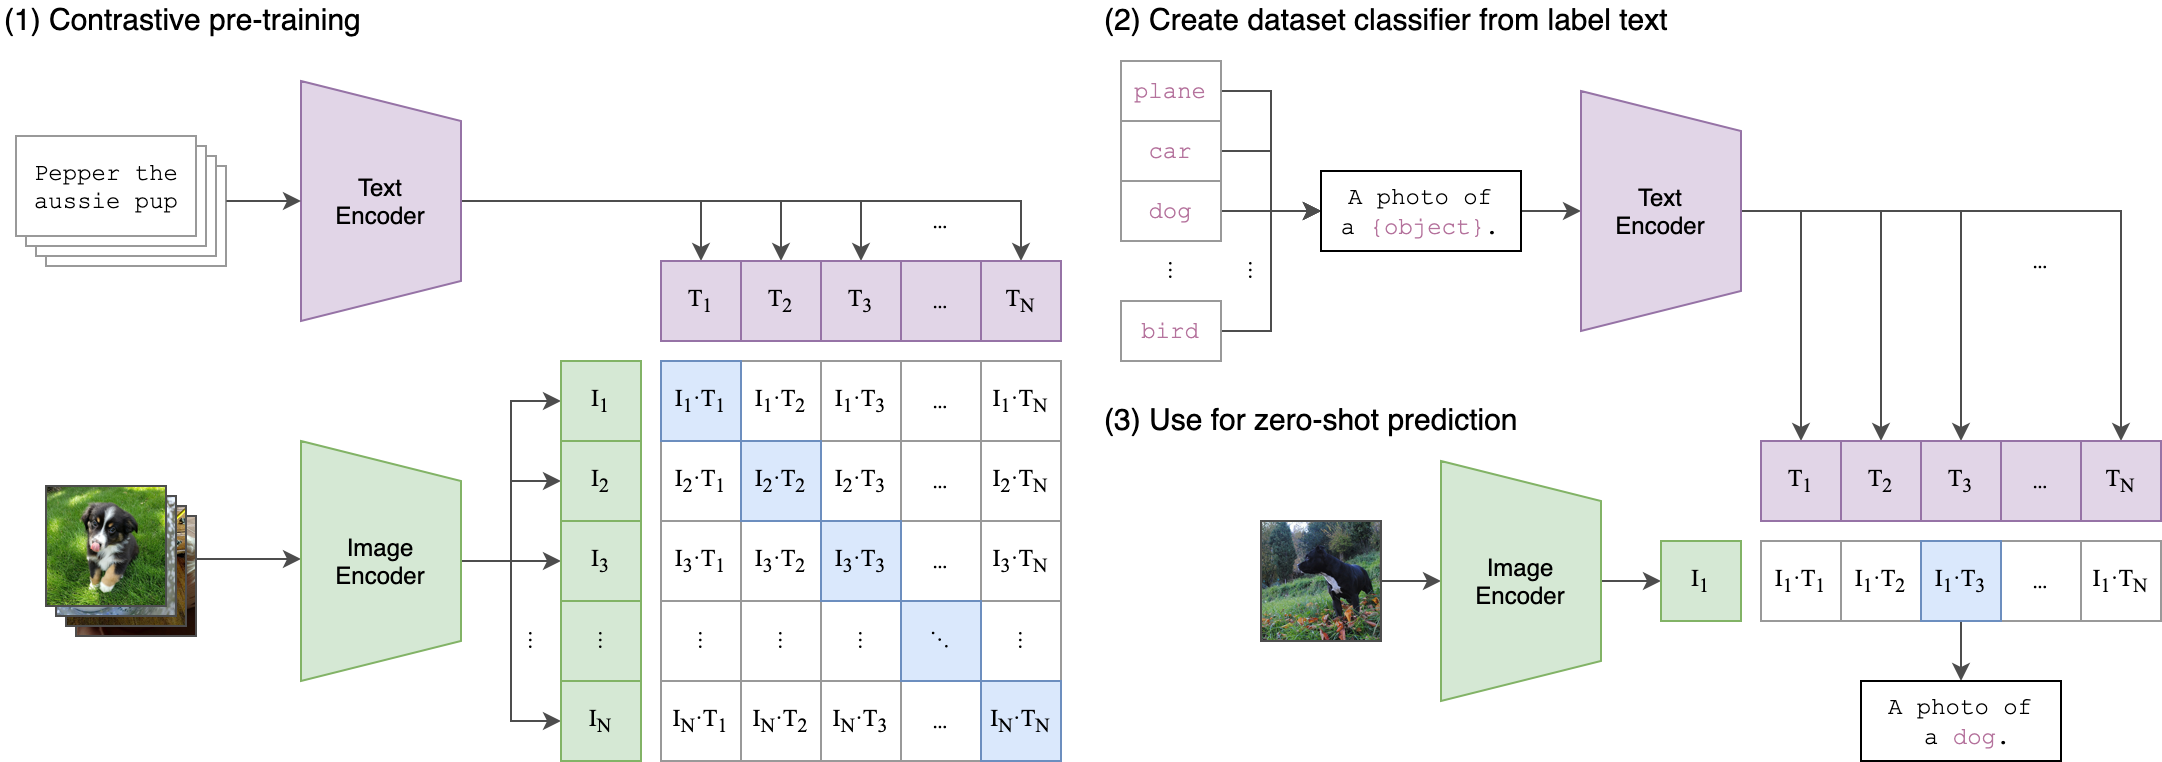
\includegraphics[width=0.8\linewidth]{CLIP.png}
  \caption{Architecture of CLIP from \cite{radford2021learning}.}
  \label{fig:CLIP}
\end{figure}


As presented in Figure \ref{fig:CLIP}, CLIP works by taking  textual prompts and images as inputs, which it encodes respectively. It then maps them to a space which enables to compute the distance between each text prompt and image prompt. For the zero-shot classification task, we want to pair the closest images and texts. CLIP outputs the probability that each image belongs to each class, making it relatively simple to extract the class with the highest probability for each image.

\paragraph{Hyperparameters} For the implementation of CLIP, besides the original repository provided by OpenAI \parencite{openai2022clip-repo}, we also took inspiration from \parencite{pinecone2022clip1,pinecone2022clip2}. We chose the pretrained CLIP model \texttt{clip-vit-base-patch32}\footnote{\url{https://huggingface.co/openai/clip-vit-base-patch32}} and it uses a ViT-B/32 Transformer architecture \parencite{dosovitskiy2020image} as an image encoder and uses a masked self-attention Transformer as a text encoder, with default hyperparameters.


%add brackets around specification/paraphrasing and fix format/colours
\begin{table}[ht]
    \centering
    \begin{tabular}{c p{7cm} p{7cm}}
        \rowcolor{lightgreen} \textbf{Index} & \textbf{Prompt} & \textbf{Example} \\ \hline
        \multicolumn{3}{c}{\textbf{Specification prompts}} \\
        \rowcolor{lightgreen} 0 & class name & “comic”\\
        \rowcolor{lightgreen} 1 & “an image of a” + class name & “an image of a comic” \\
        \rowcolor{lightgreen} 2 & noun phrase & “traditional comic”\\
        \rowcolor{lightgreen} 3 & adjective 1 + adjective 2 + class name & “entertaining traditional comic” \\
        \rowcolor{lightgreen} 4 & disjunction of noun phrases & “adventure comic or humour comic or superhero comic or war comic” \\
        \rowcolor{lightgreen} 5 & noun phrases separated by commas & “adventure comic, humour comic, superhero comic, war comic” \\
        \rowcolor{lightgreen} 6 & “This” + class name + verb + preposition & “This comic is a story told with successive images” \\
        \multicolumn{3}{c}{\textbf{Paraphrasing prompts}} \\
        \rowcolor{lightgreen} 7 & class guidelines & “Comic or Satirical Drawing: Any humour or entertainment drawing. Could include text bubbles or text descriptions. Could be both one image or multiple to create a mini graphic novel.” \\
        \rowcolor{lightgreen} 8 & class name + “:” + adapted Cambridge definition & “comic: a set of stories told in pictures with a small amount of writing” \\
        \rowcolor{lightgreen} 9 & adapted Cambridge definition & “a set of stories told in pictures with a small amount of writing” \\
        \rowcolor{lightgreen} 10 & class name + “:” + Cambridge definition & “comic: a set of stories told in pictures with a small amount of writing” \\
        \rowcolor{lightgreen} 11 & Cambridge definition & “a set of stories told in pictures with a small amount of writing” \\
        \rowcolor{lightgreen} 12 & ChatGPT analogy of the class to the prompt \textit{Give me an analogy that captures the essence of a comic} & “A comic is like a rollercoaster ride for your imagination. Just as a rollercoaster takes you on a thrilling journey with its twists, turns, and unexpected drops.” \\
    \end{tabular}
    \caption{Prompt variations for zero-shot classification using CLIP with examples on the class \textit{comic}.}
    \label{tab:prompt_variations}
\end{table}


\subsection{Prompting CLIP for zero-shot image classification}

We are particularly interested in determining how to best prompt the model to gain insights on its true potential and optimize its performance. To have a first glimpse at how CLIP behaves, we prompted it using only the eight class names. Then, we curated a list of prompts from simple to more complex, presented in Table \ref{tab:prompt_variations}. We distinguish specification prompts from paraphrasing prompts:

\begin{itemize}
    \item \textbf{Specification prompts}: They focus on providing specific details and characteristics related to the target class. They aim to specify attributes, features, and categorizations associated with the given class.
    \item \textbf{Paraphrasing prompts}: They restate, define the target class in alternative ways. They aim to convey the essence or definition using different linguistic constructs, promoting a varied understanding of the same concept.
\end{itemize}


The prompt variations were carefully designed with the intention to answer the following questions:
\begin{enumerate}
    \item How sensitive is CLIP to small changes in wording, connectors, punctuation and length of prompt?
    \item Does CLIP understand nuances of words? Can it associate them to a general concept?
    \item What is the prompt pattern that yields the best results?
    \item How confident is CLIP when making correct and incorrect predictions?
\end{enumerate}

For each one of the thirteen experiments, the same prompt variation was consistently applied on every class, except for the last experiment, where we prompted CLIP with the best performing prompt on each class. We are interested in the progression of the F-score per class. The curve should follow a consistent pattern over all classes, which should also be consistent with the average accuracy curve. 

\subsubsection{Results}
Our initial emphasis is on the simplest prompt, namely the \textit{class names}. This prompt type yields an average accuracy of \textbf{61.93\%}, with the lowest F-score being 0\% for the class \textit{title}, as illustrated in Figure \ref{fig:CLIP-zero-shot-class-name-A}. In fact, as can be observed in Figure \ref{fig:CLIP-zero-shot-class-name-B}, all titles are misclassified as logos.

\begin{figure}[ht]
    \centering
    \begin{subfigure}{0.47\textwidth}
        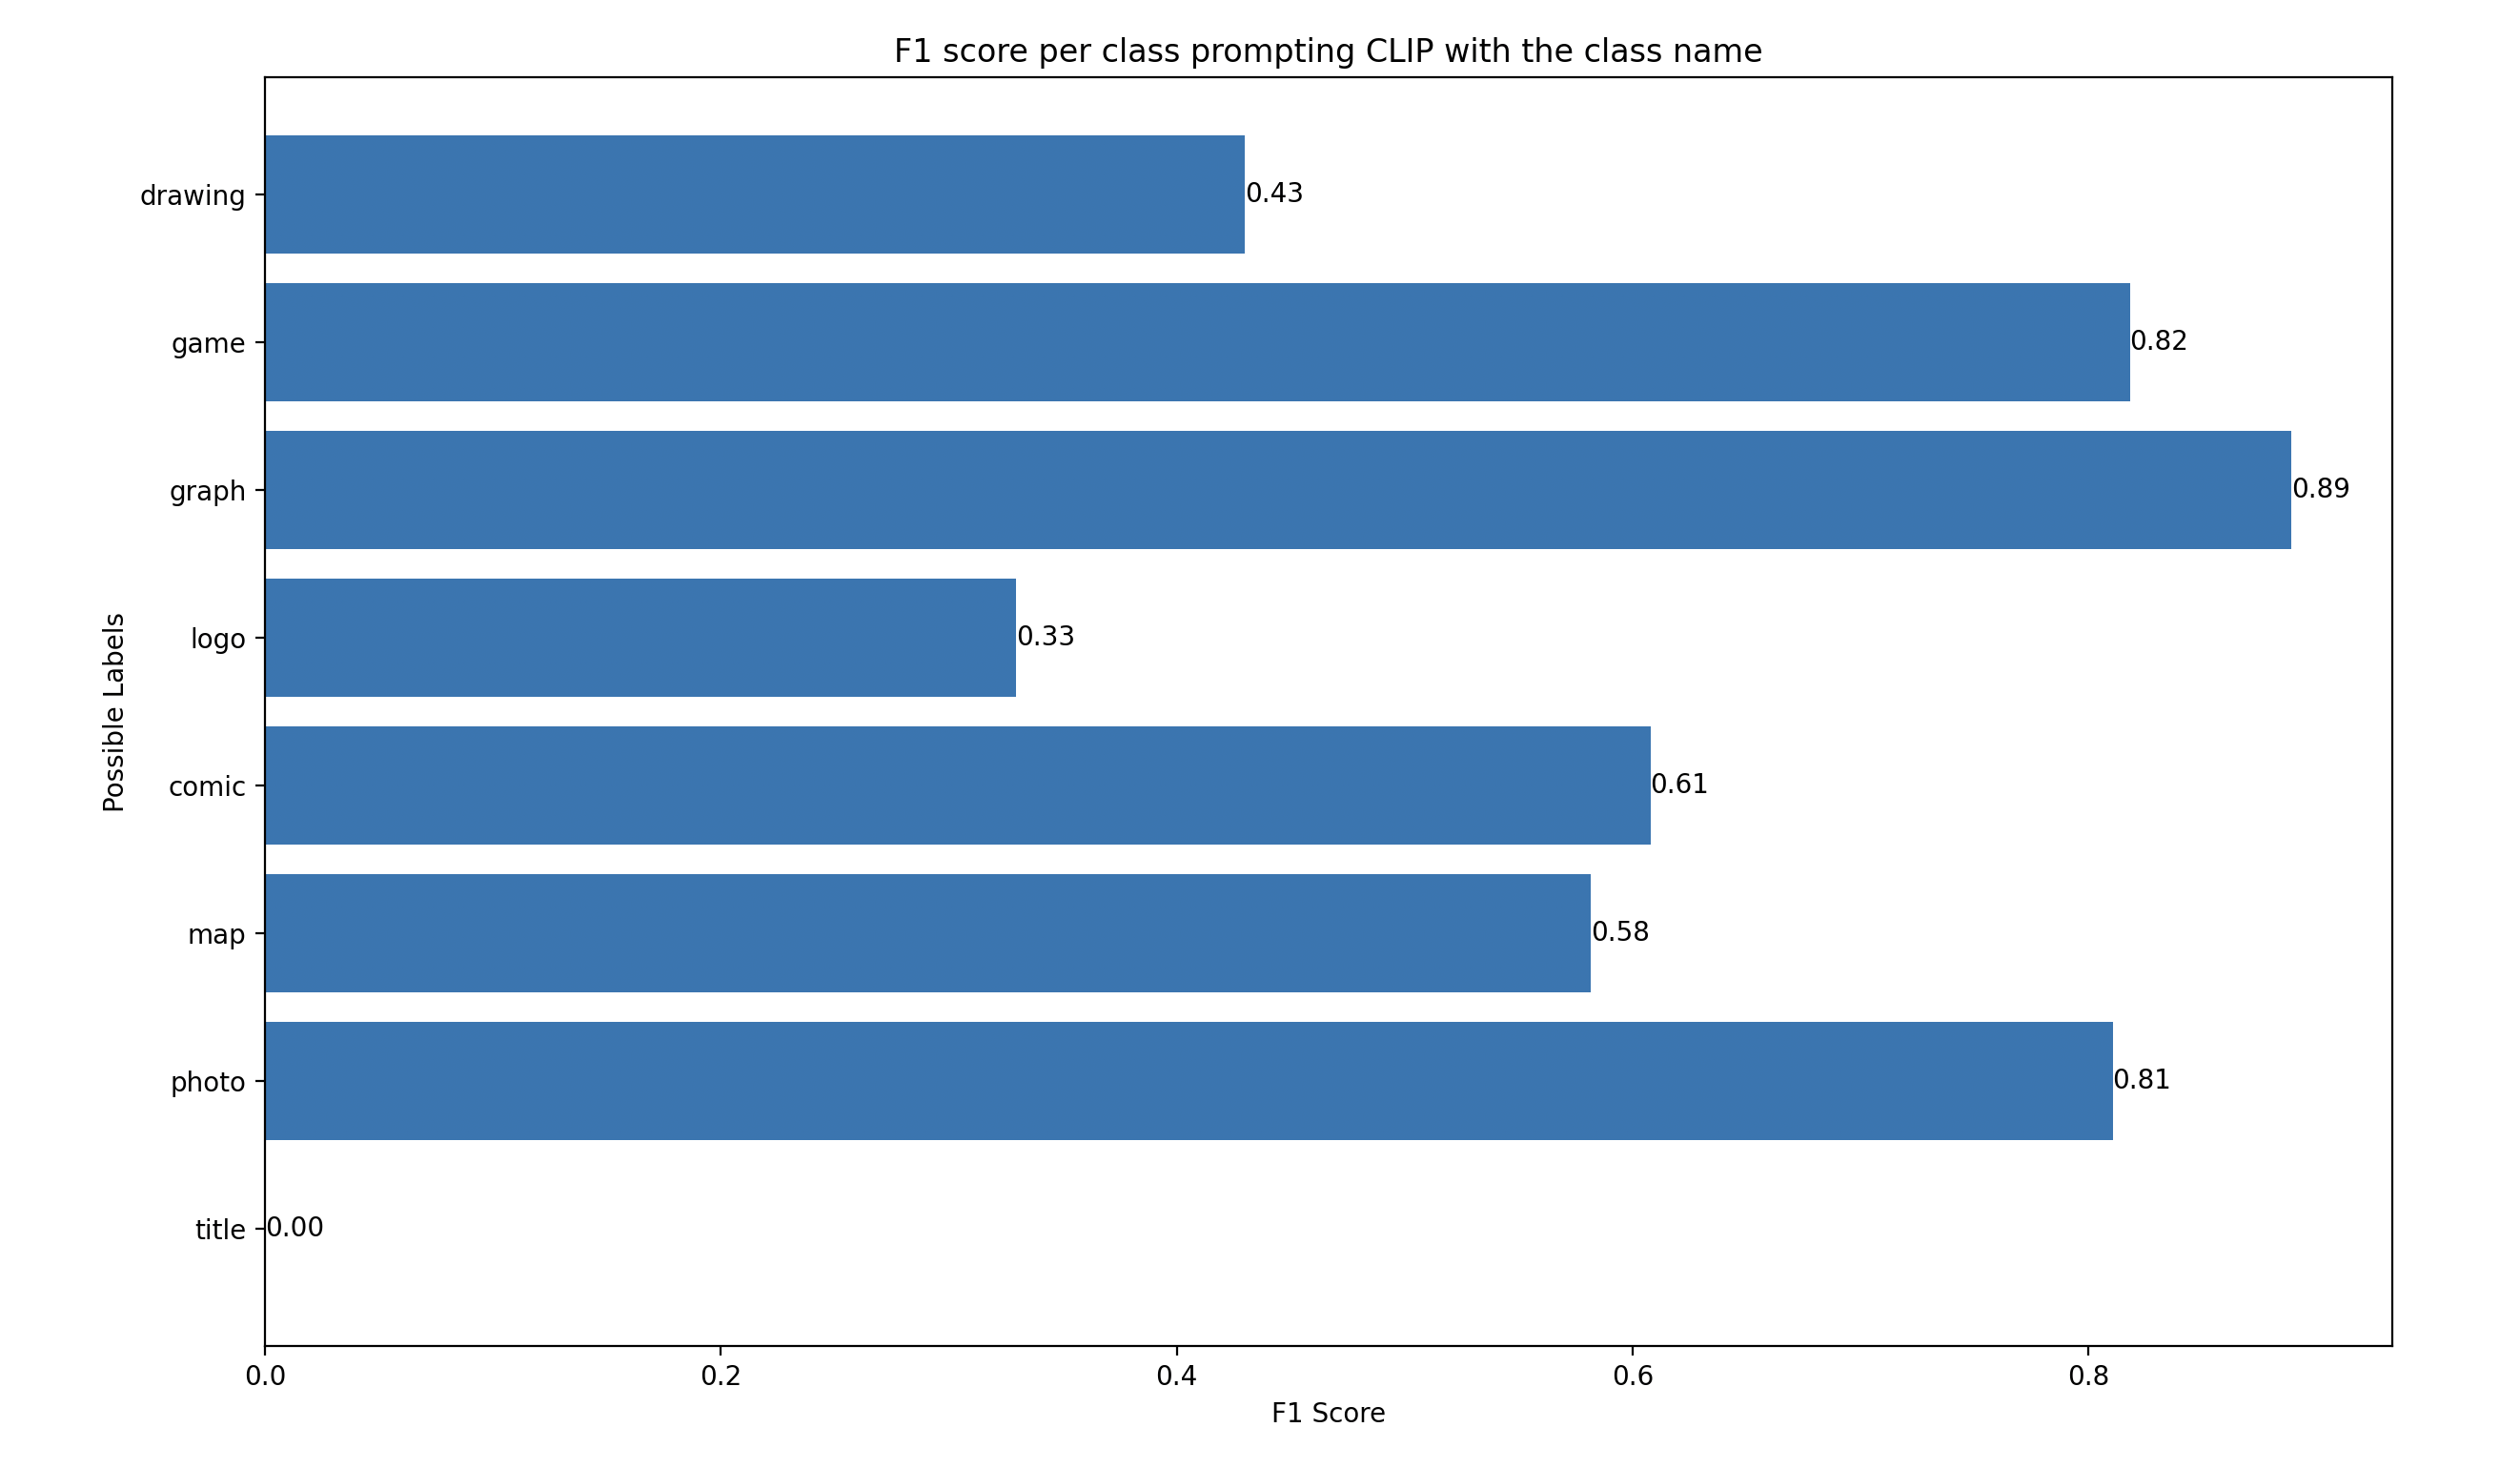
\includegraphics[width=\linewidth]{Images/CLIP-results/F1-score-CLIP-p0.png}
        \caption{F-score per class.}
        \label{fig:CLIP-zero-shot-class-name-A}
    \end{subfigure}
    % \hfill
    \begin{subfigure}{0.47\textwidth}
        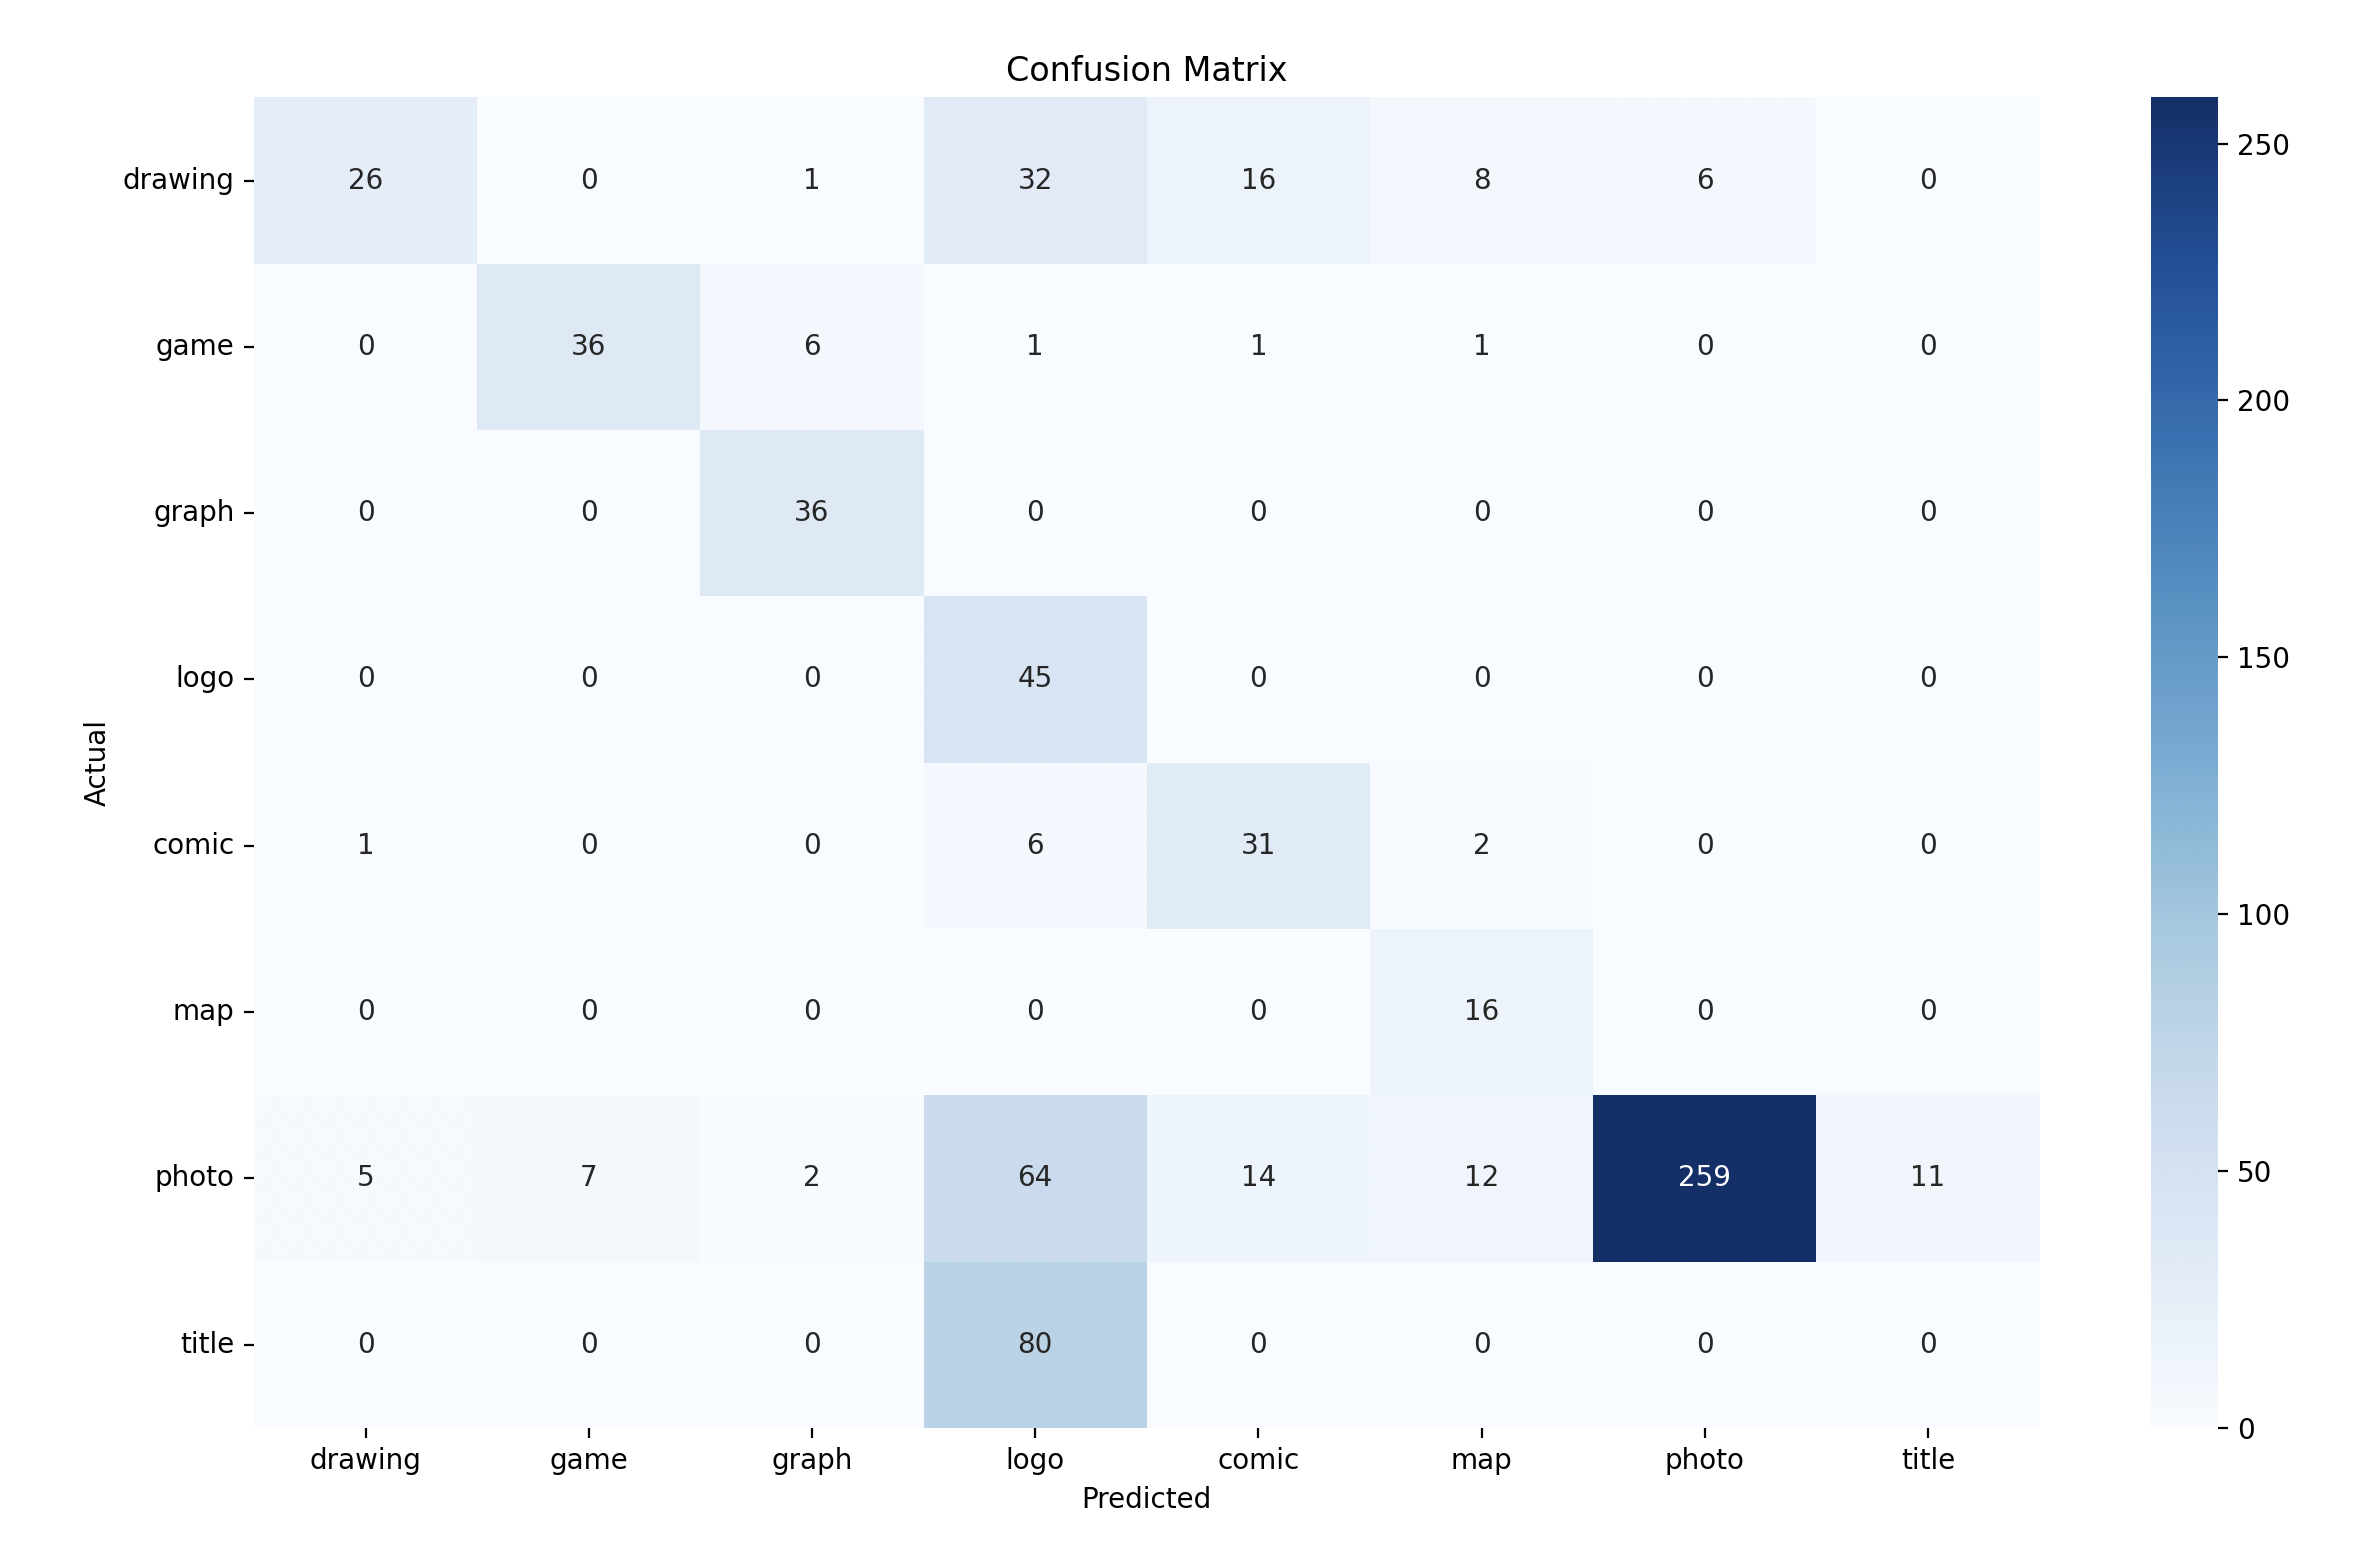
\includegraphics[width=\linewidth]{CM-CLIP.png}
        \caption{Confusion matrix.}
        \label{fig:CLIP-zero-shot-class-name-B}
    \end{subfigure}
    \caption{CLIP zero-shot classification results on \textit{class name} prompt.}
    \label{fig:CLIP-zero-shot-class-name}
\end{figure}


This result is not surprising given that the images for this class are mainly title-font single letters and not complete titles. We can safely affirm that this low score is due to the class name being inaccurate, more than the capability of the model. As presented in Figure \ref{fig:F1-score-difference}, changing the prompt from \textit{title} to \textit{title-font letter} increases the F-score from 0\% to 83\%.


We notice in Figure \ref{fig:CLIP-zero-shot-class-name-B} that the majority of misclassifications are false positive for the class \textit{logo}. Mostly images labelled as \textit{drawing}, \textit{photo}, and \textit{title} are misclassified as a \textit{logo}. We can see a few examples of this type of misclassification in Figure \ref{fig:logo_FPs}.

\clearpage

%change layout of table 3.2. it doesn't look good
\begin{figure}[ht]
    \centering

    \begin{minipage}[5cm]{0.3\textwidth}
        \centering
        \begin{subfigure}{3.5cm}
            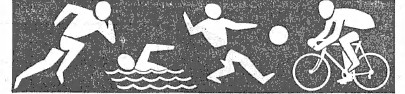
\includegraphics[width=\linewidth]{Images/logo FPs/drawings/EXP-1972-12-02-a-i0308.jpg}
            
        \end{subfigure}

        \begin{subfigure}{3.5cm}
            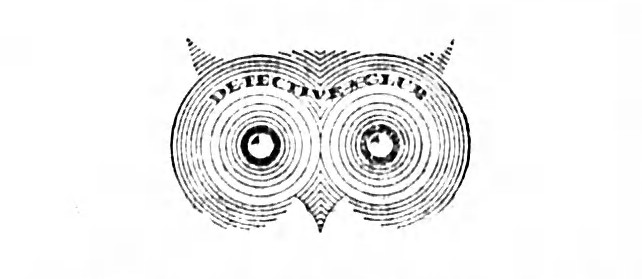
\includegraphics[width=\linewidth]{Images/logo FPs/drawings/GDL-1951-10-24-a-i0014.jpg}
            
        \end{subfigure}

        \begin{subfigure}{3.5cm}
            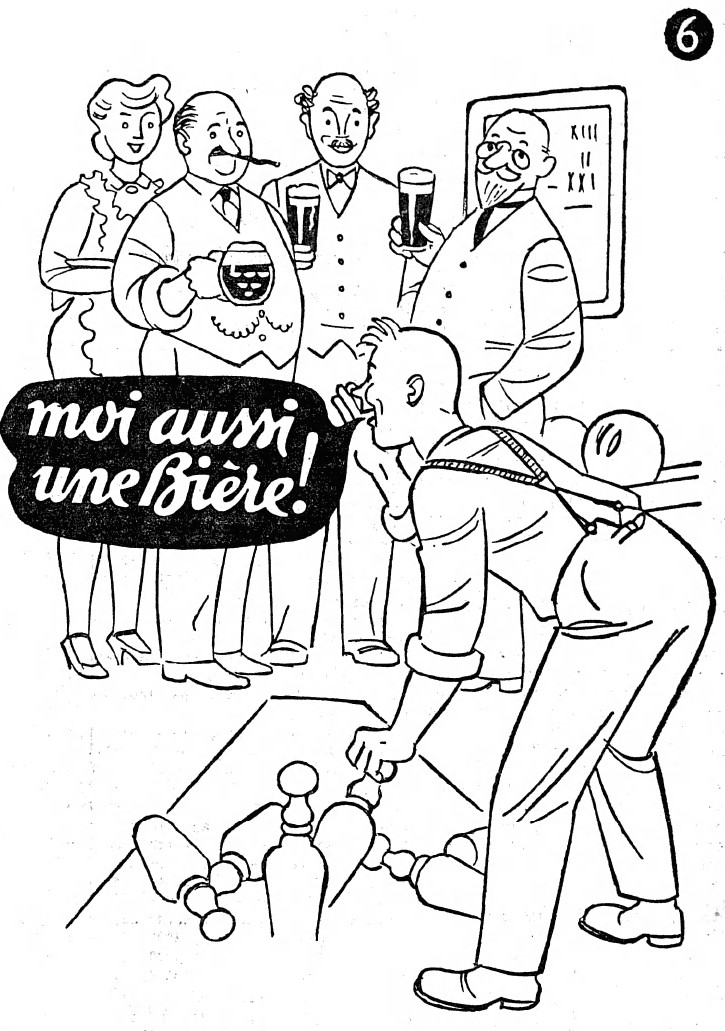
\includegraphics[width=\linewidth]{Images/logo FPs/drawings/IMP-1955-01-31-a-i0053.jpg}
            \caption{Drawings}
        \end{subfigure}
    \end{minipage}%
    \hfill
    \begin{minipage}[5cm]{0.3\textwidth}
        \centering
        \begin{subfigure}{3cm}
            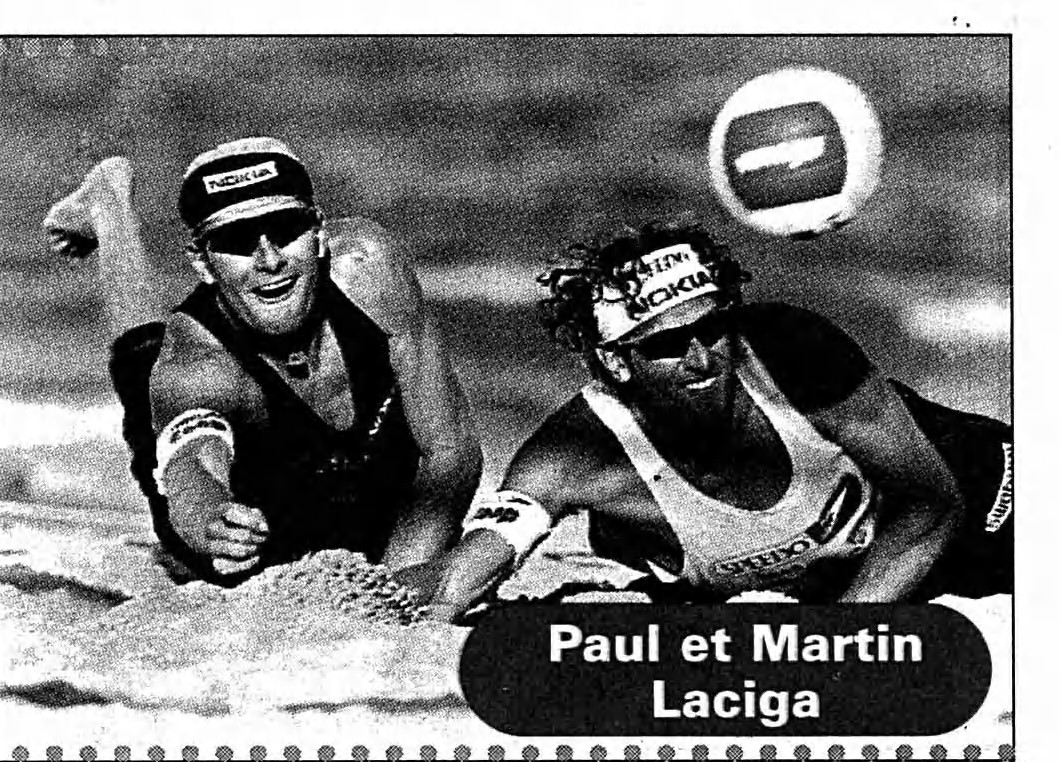
\includegraphics[width=\linewidth]{Images/logo FPs/photos/EXP-2000-09-13-a-i0271.jpg}
            
        \end{subfigure}

        \begin{subfigure}{3cm}
            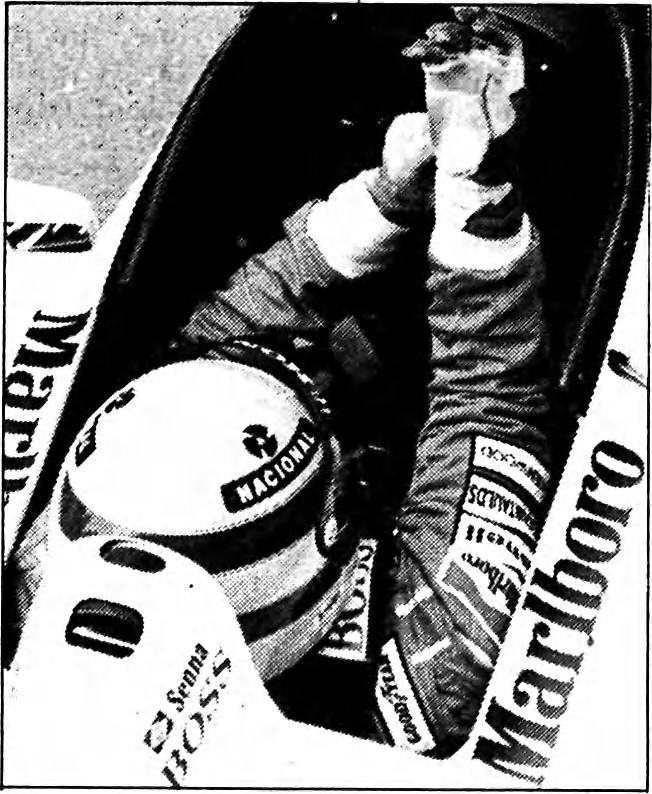
\includegraphics[width=\linewidth]{Images/logo FPs/photos/GDL-1993-03-13-a-i0130.jpg}
            
        \end{subfigure}

        \begin{subfigure}{3cm}
            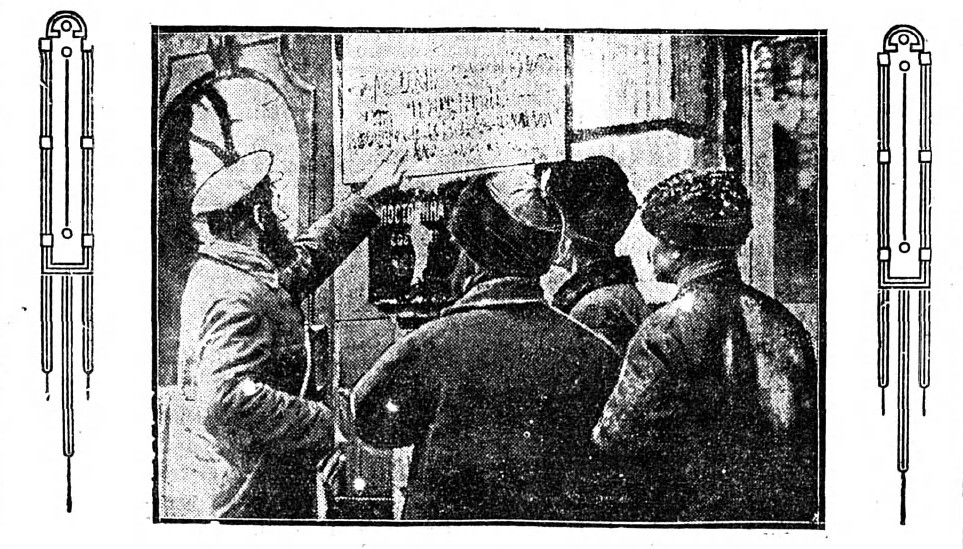
\includegraphics[width=\linewidth]{Images/logo FPs/photos/IMP-1929-08-23-a-i0002.jpg}
             \caption{Photos}
        \end{subfigure}
    \end{minipage}%
    \hfill
    \begin{minipage}[5cm]{0.3\textwidth}
        \centering
        \begin{subfigure}{1.9cm}
            
\includegraphics[width=\linewidth]{Images/logo FPs/titles/LCE-1906-07-25-a-i0010.jpg}
            
        \end{subfigure}

        \begin{subfigure}{2cm}
            
\includegraphics[width=\linewidth]{Images/logo FPs/titles/LCE-1921-12-09-a-i0059.jpg}
            
        \end{subfigure}

        \begin{subfigure}{1.7cm}
            
\includegraphics[width=\linewidth]{Images/logo FPs/titles/LCE-1942-05-20-a-i0019.jpg}
             \caption{Titles}
        \end{subfigure}
    \end{minipage}

    \caption{Examples of false positives for \textit{logo} using the \textit{class name} prompt.}
    \label{fig:logo_FPs}
\end{figure}
%FLAMINGO also misclassifies a lot logo! Develop on this in the comparison. 


Moving forward to the next experiments, we obtain the holistic results for all prompts presented in Figure \ref{fig:CLIP-zero-shot-13}, which will enable us to answer the questions previously stated.
 
\begin{figure}[ht]
    \centering
    \begin{subfigure}{0.47\textwidth}
        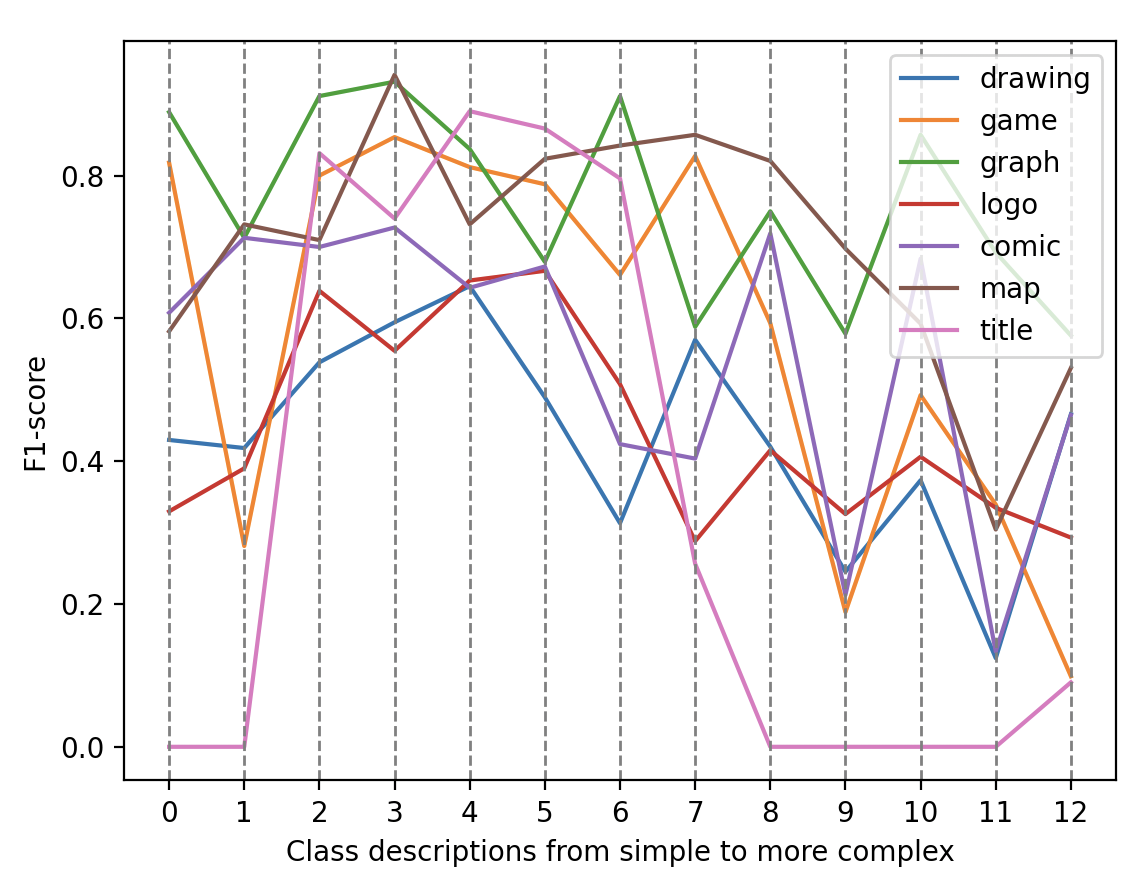
\includegraphics[width=\linewidth]{Images/CLIP-results/CLIP-holostic-res.png}
        \caption{F1 per class for each one of the 13 prompts.}
        \label{ig:CLIP-zero-shot-13-A}
    \end{subfigure}%
    \hspace{0.06\textwidth}% Adjust the length to control the padding
    \begin{subfigure}{0.47\textwidth}
        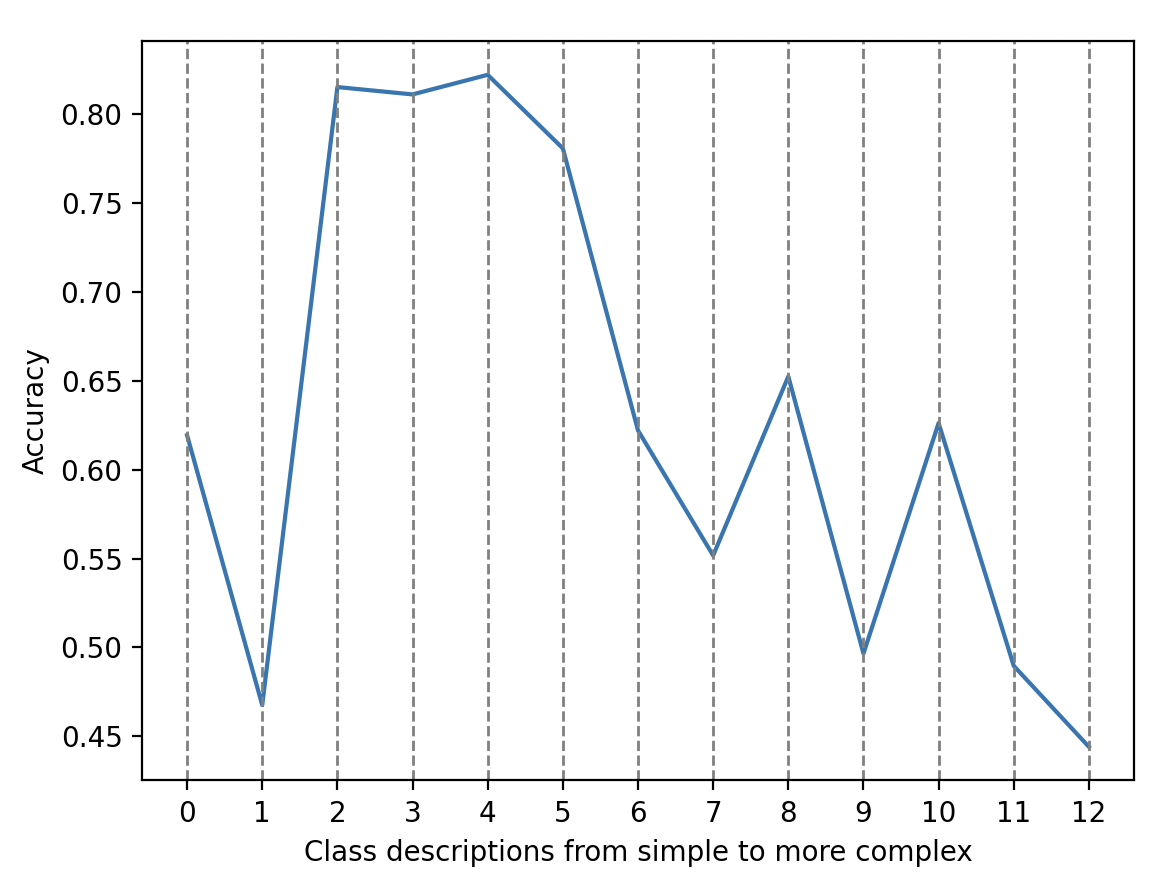
\includegraphics[width=\linewidth]{Images/CLIP-results/CLIP-holistic-avg-acc.png}
        \caption{Average accuracy per prompt.}
        \label{ig:CLIP-zero-shot-13-B}
    \end{subfigure}
    
    \hspace{0.06\textwidth}% Add more padding if needed
    
    \begin{subfigure}{0.47\textwidth}
        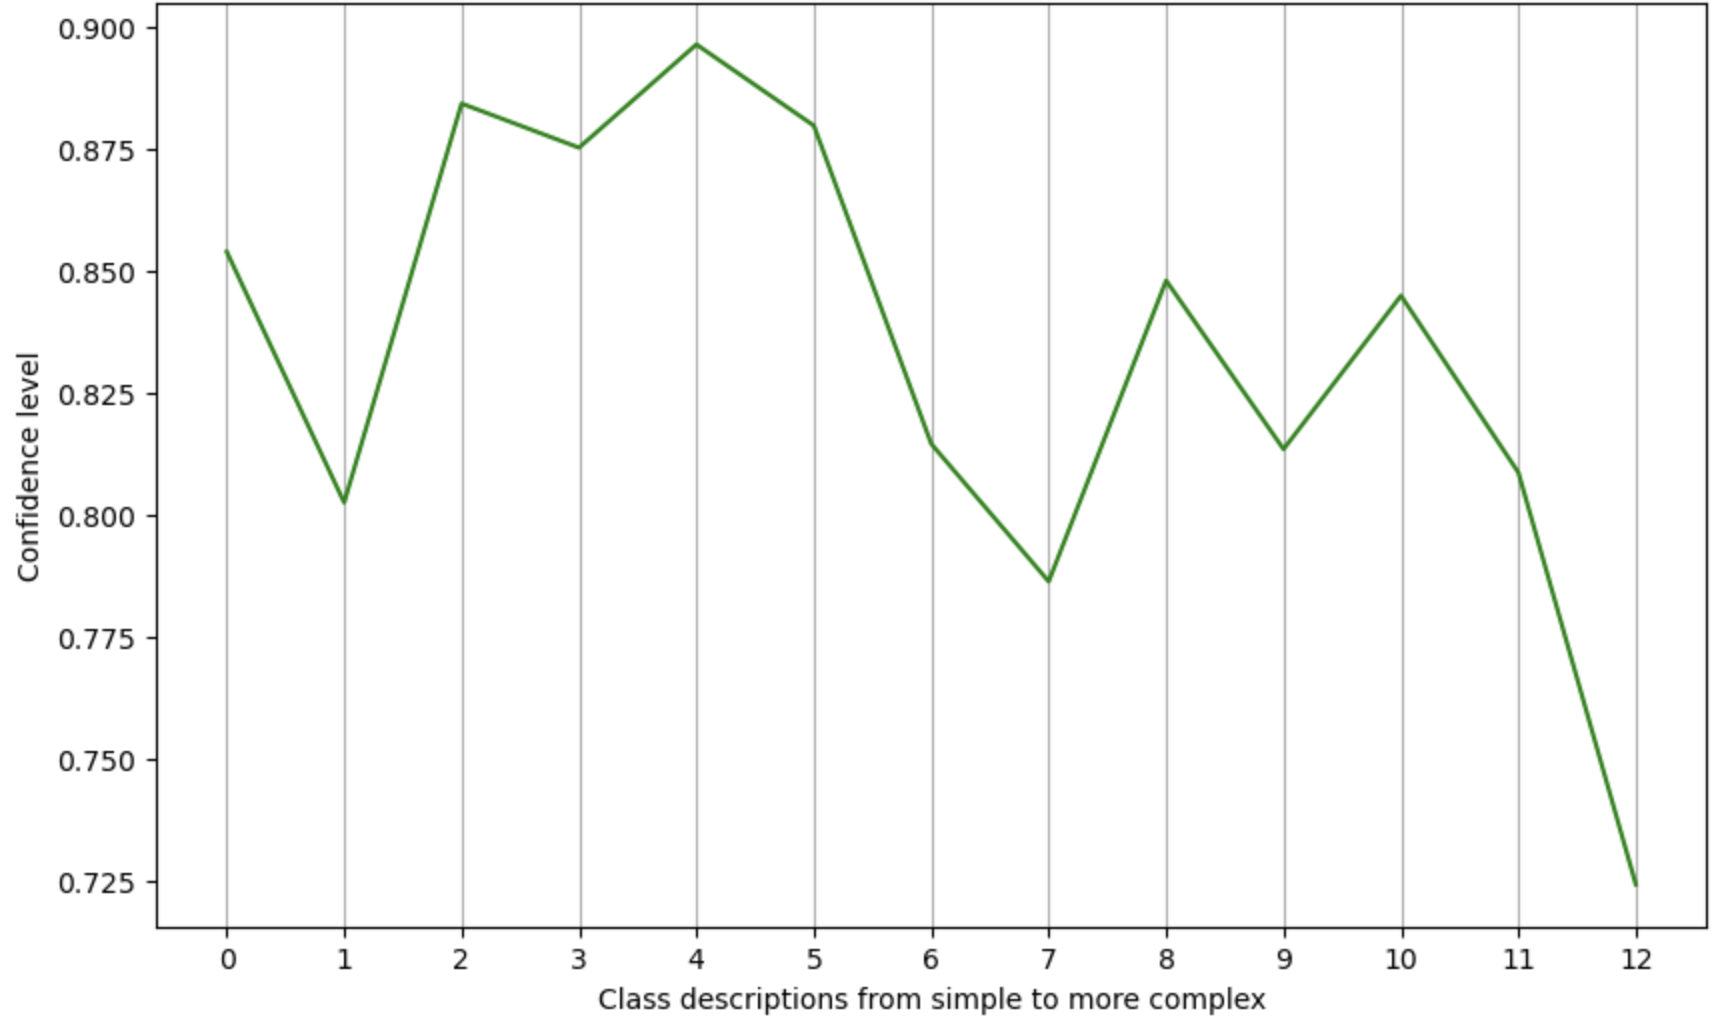
\includegraphics[width=\linewidth]{Images/CLIP-results/Confidence.png}
        \caption{Average confidence level per prompt.}
        \label{ig:Confidence-levels}
    \end{subfigure}
    
    \caption{CLIP zero-shot classification results on 13 prompt variations.}
    \label{fig:CLIP-zero-shot-13}
\end{figure}

Looking at Figure \ref{ig:CLIP-zero-shot-13-A}, we notice a general pattern in the F1 of the classes, revealing the best-performing prompts. This pattern is well reflected in Figure \ref{ig:CLIP-zero-shot-13-B}, illustrating the average accuracy per prompt over all classes. Moreover, it overlaps with the pattern observed on the confidence level. This behaviour is favourable, as the model's confidence level is directly correlated to its accuracy.

We notice that CLIP works well on the four specification prompts summarised in Table \ref{tab:best-prompts} along with their performance. The structure of these prompts is simpler than the paraphrasing prompts. The idea is to concisely express the essence of the class, exhaustively but with as less wording as possible.
Moreover, CLIP is sensitive to changes in punctuation and connectors, as the \textit{disjunction of noun phrases} prompt performs better than the \textit{noun phrases separated by comas} prompt, even though the same noun phrases are used for both prompts.


Finally, CLIP is able to understand nuances of words as long as they are not too abstract. It can associate a word to a general concept if the word can be put out of its context and still hold the same meaning. As seen in Figure \ref{fig:CLIP-zero-shot-13}, it performs poorly on the metaphorical definitions of the classes, which correspond to prompt 12.


\begin{table}[h]
    \centering
    \arrayrulecolor{white}
    \begin{tabular}{lr}
    \rowcolor{gray!25}
        \textbf{Prompt structure} & \textbf{Average accuracy} \\
        noun phrase & 79.45\% \\
        adjective 1 + adjective 2 + noun phrase & 78.21\% \\
        disjunction of noun phrases & \bf 82.21\% \\
        noun phrases separated by comas & 78.07\%\\
    \end{tabular}
    \caption{Average accuracy of the best performing prompt variations.}
    \label{tab:best-prompts}
\end{table}

The best average accuracy is \textbf{82.21\% }, when prompting CLIP with disjunctions of noun phrases. 
\\Can we confidently assert that the \textit{disjunction of noun phrases} prompt generally yields the best performance? To answer this question, we tried a new variation where we took the best performing prompt for each class. For every class, Figure \ref{fig:F1-score-difference} illustrates the difference in F-score between each type of variation and prompt 0, i.e. the class names. We notice that the highest increase always occurs when prompting CLIP with one of the four specification prompts, indexed from 2 to 5 in Figure \ref{fig:F1-score-difference}. 


\begin{figure}[ht]
  \centering
  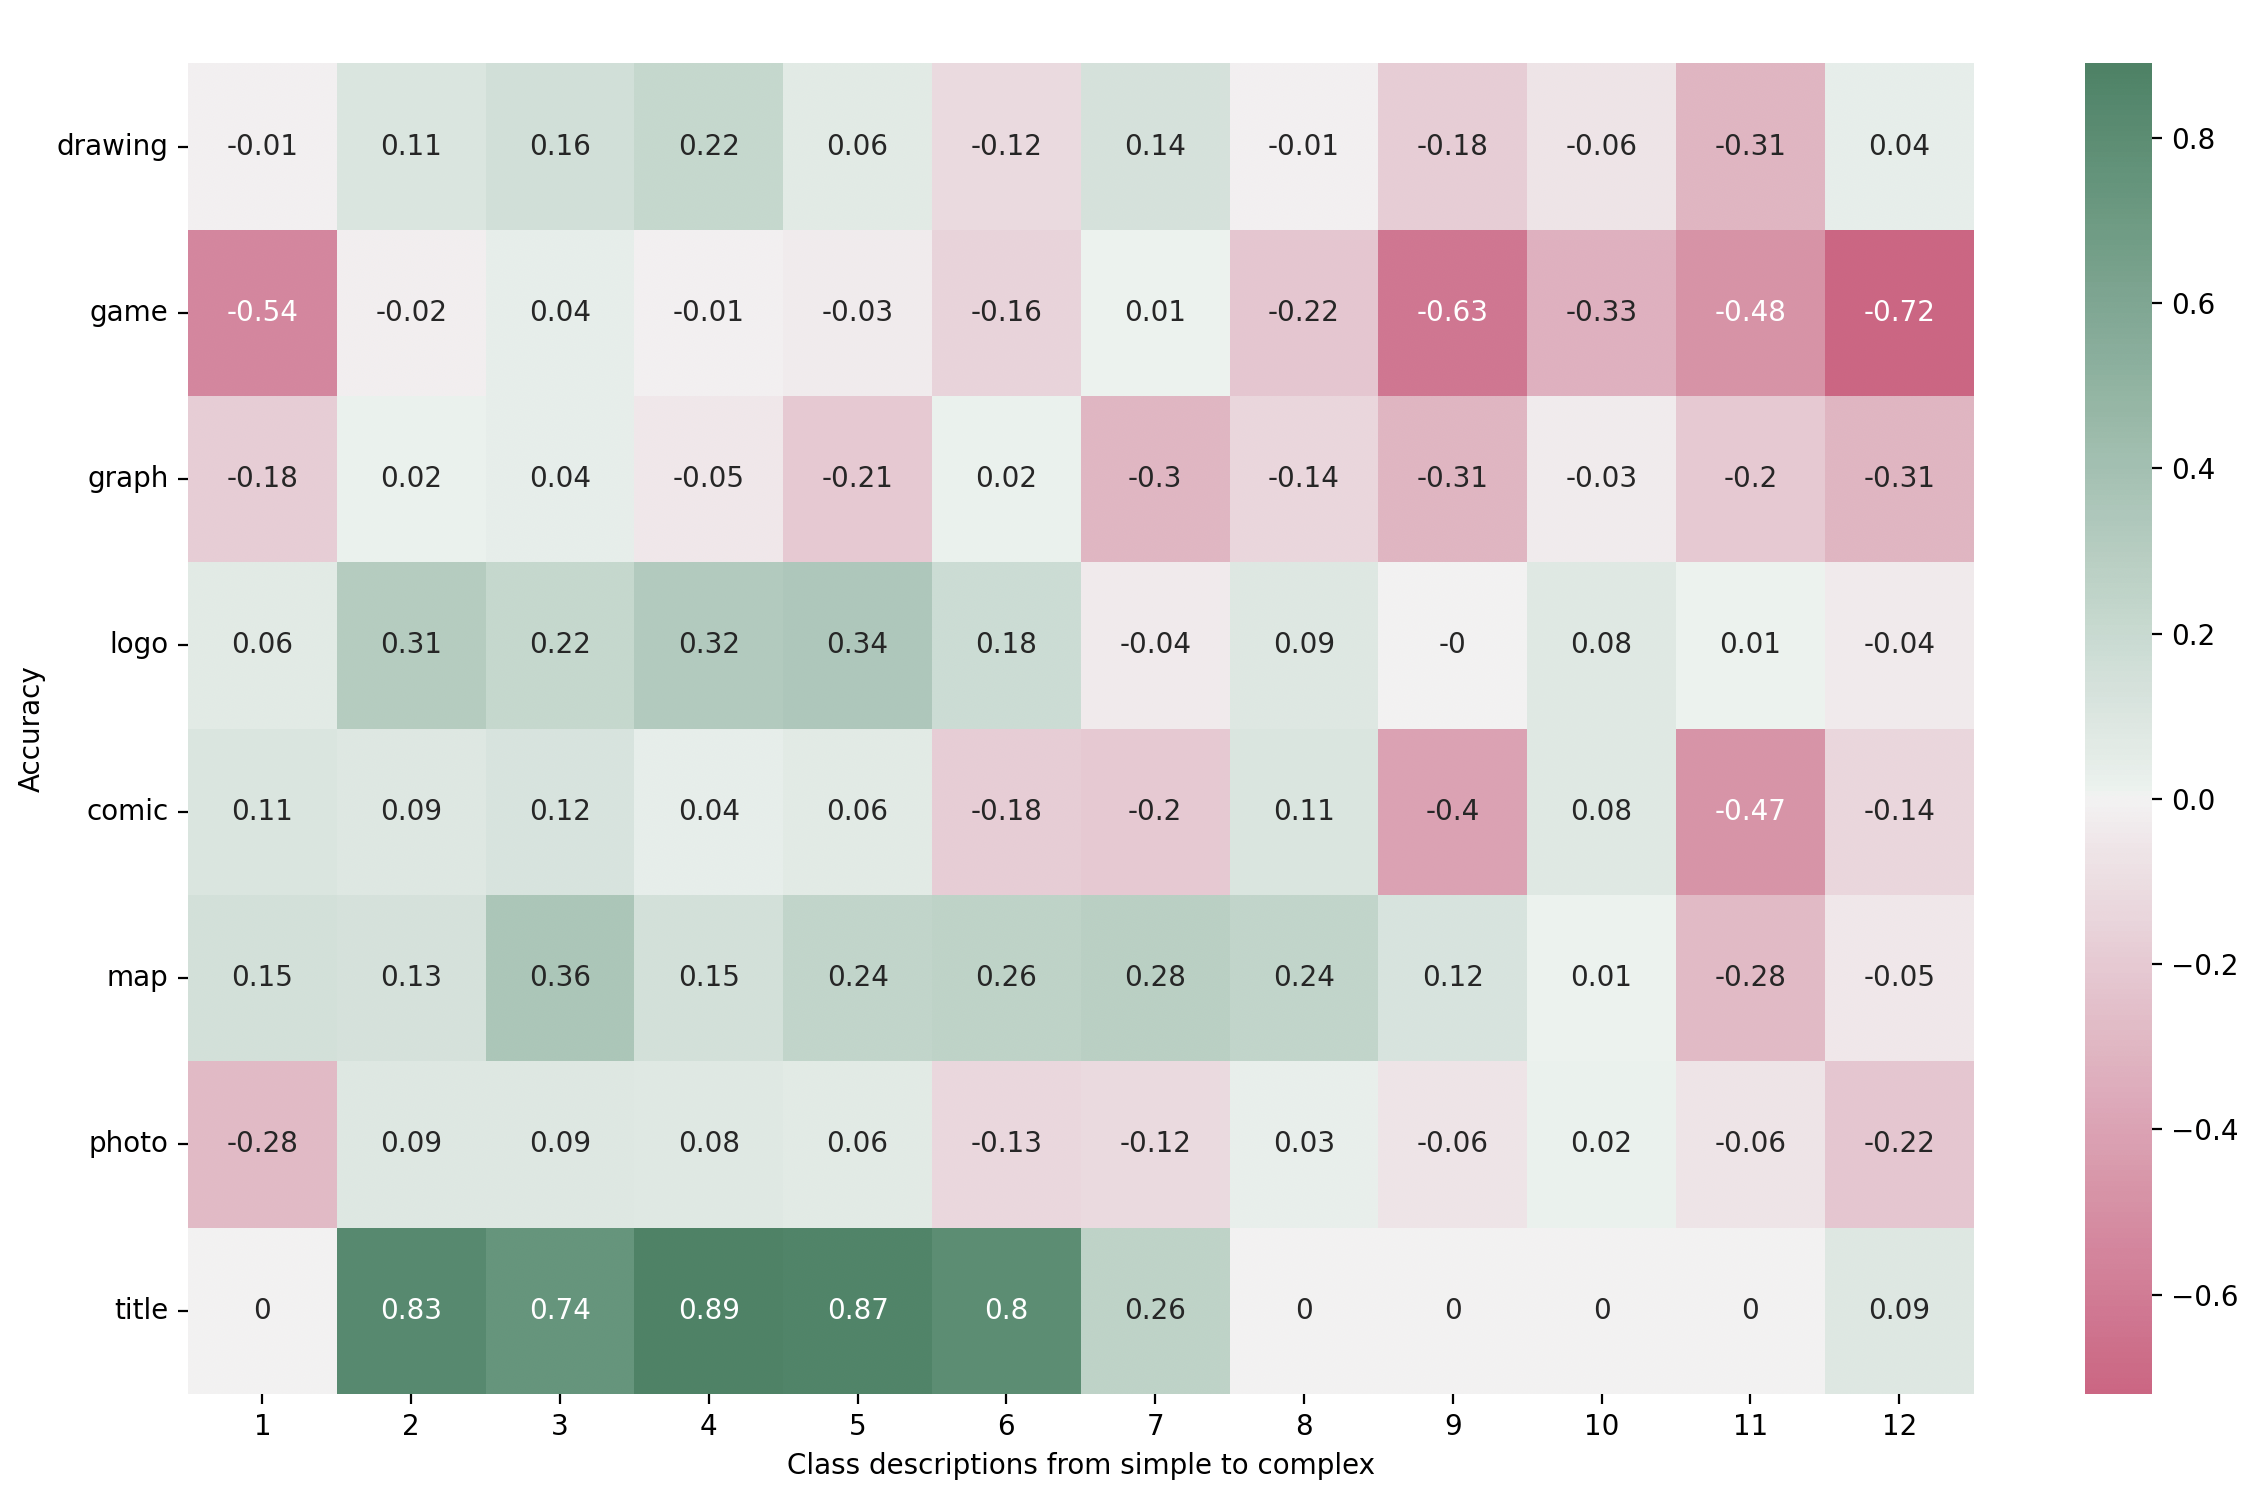
\includegraphics[width=0.7\linewidth]{Images/CLIP-results/F1-score difference.png}
  \caption{Differences in F-score between \textit{class name} prompt and other prompt variations.}
  \label{fig:F1-score-difference}
\end{figure}

The results show that the average accuracy stagnates in the range of 82\%. Therefore, any of the four specification prompts is well understood by CLIP. Moreover, \textbf{CLIP performs significantly better when the specifications are exhaustive}.


We are left with the task of narrowing down the options and getting a more specific guideline to prompt CLIP optimally. The hypothesis that we will support in the following section is that the difference in performance between the specification prompts depends on factors outside the grammatical structure of the prompt. 

We, thus, mainly focus on the influence of lexical choices. In order to do this, we study misclassifications and experiment on a selection of prompts by strategically altering the lexicon and analysing the results.

% \clearpage



\subsection{Experimenting with lexical choices}

In this section, we have a closer look at the most recurrent misclassifications with the best results achieved yet, namely prompting CLIP with disjunction of noun phrases. We choose to focus specifically on the classes \textit{comic} and \textit{drawing} due to their interesting relationship. A \textit{comic} is a subset of drawings, as it involves creating images through the art of drawing. However, not all drawings can be classified as comics, as comics typically involve a sequential narrative format with associated text or dialogue.

\subsubsection{Results}

We notice in Figure \ref{ig:CM-A} that within the \textit{comic} class, there are ten instances of false positives of comics, marked in orange, where drawings are misclassified as comics. On the other hand, there are ten instances of false negatives of comics, marked in red, where comics are misclassified as drawings.

\begin{figure}[ht]
    \centering
    \subcaptionbox{Confusion matrix with no lexicon alteration\label{ig:CM-A}.}{%
        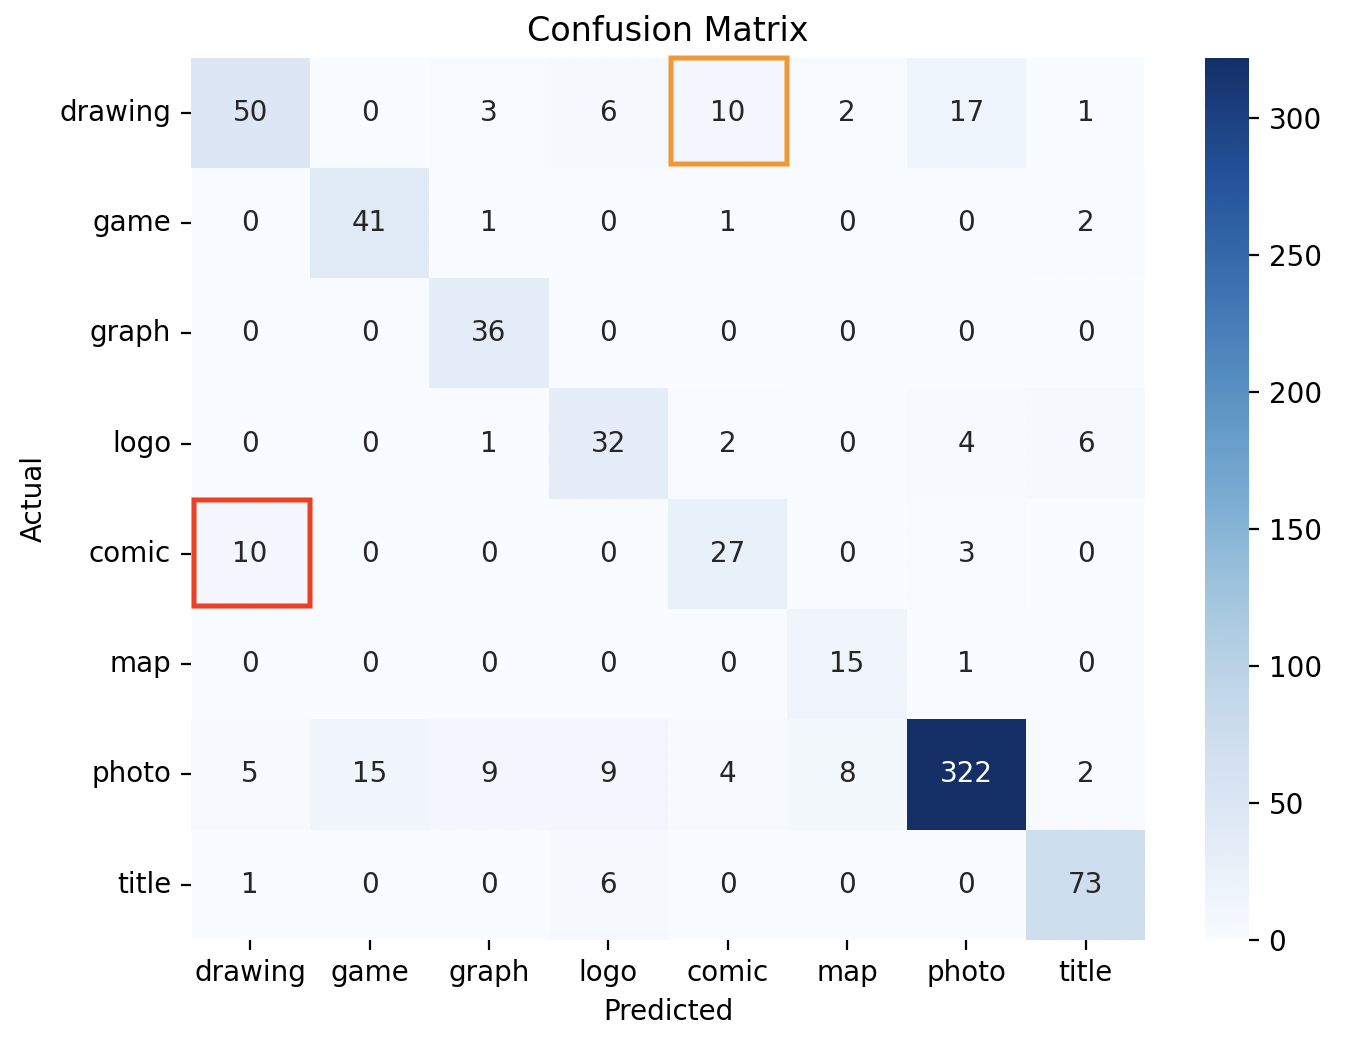
\includegraphics[width=0.31\textwidth]{Images/CLIP-results/CLIP-best-perf-CM.png}%
    }\hfill
    \subcaptionbox{Confusion matrix when specifying that a drawing does not contain text\label{ig:CM-B}.}{%
        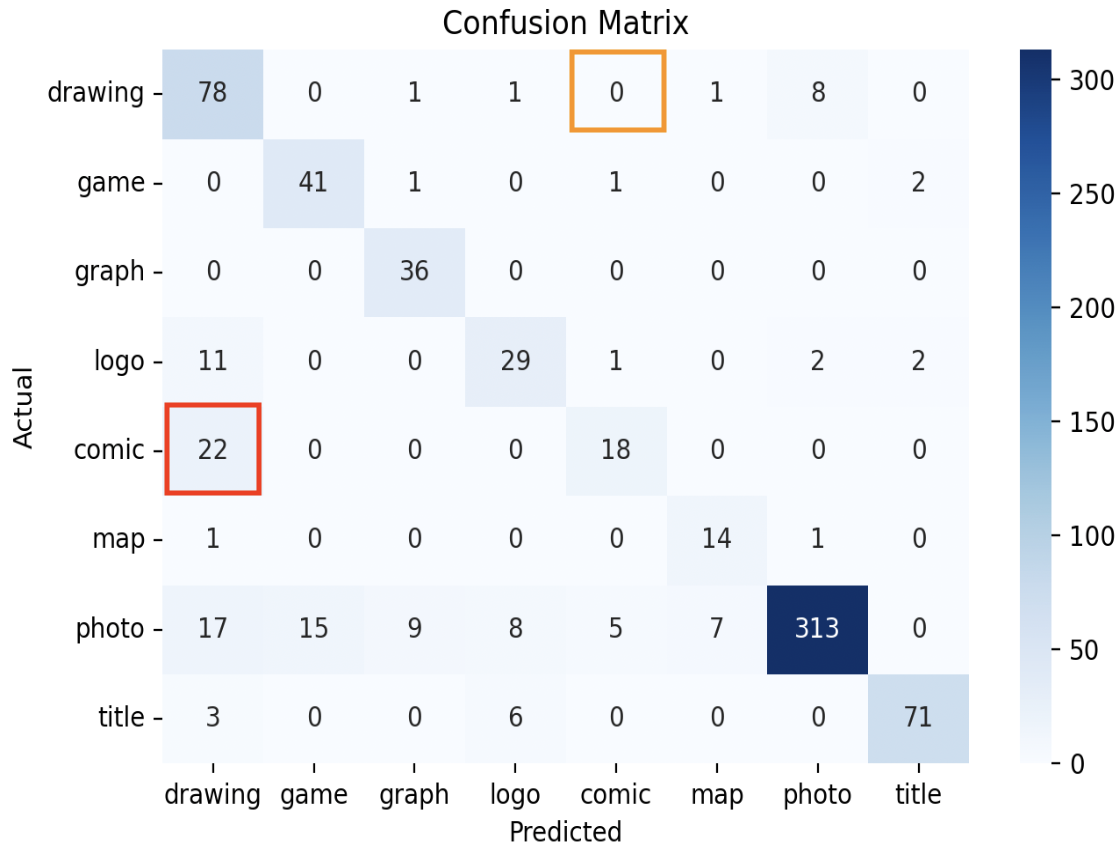
\includegraphics[width=0.31\textwidth]{Images/CLIP-results/CM-non-text.png}%
    }\hfill
    \subcaptionbox{Confusion matrix when specifying that a comic contains text\label{ig:CM-C}.}{%
        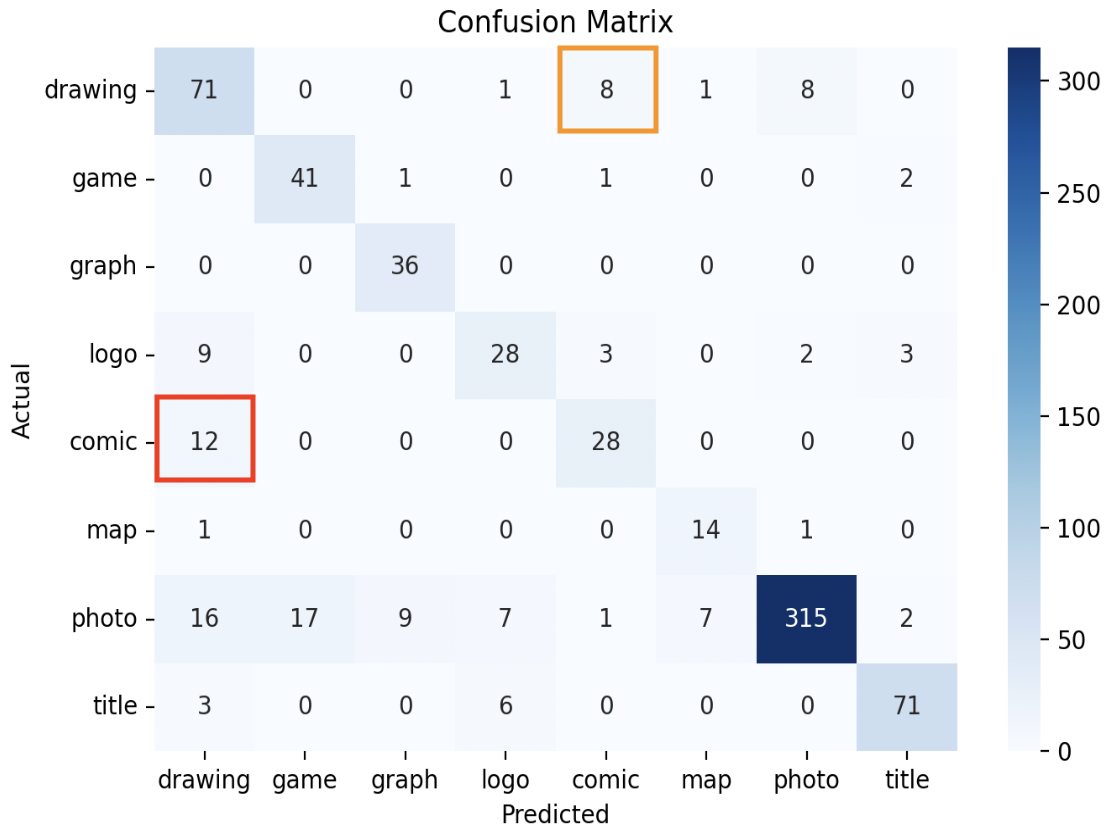
\includegraphics[width=0.31\textwidth]{Images/CLIP-results/CM-text.png}%
    }
    \caption{Progression of the confusion matrix using the \textit{disjunction of noun phrases} prompt when altering the lexicon of the prompts for \textit{comic} and \textit{drawing}.}
    \label{fig:CMs altering lexicon}
\end{figure}


To attempt fixing the false positives, we specify in the prompt for the class \textit{drawing} that a drawing does not contain text. Thus, we modify the prompt from \textit{“illustration or cartoon or caricature or descriptive drawing”} to \textit{“\underline{non-textual} illustration or cartoon or caricature or descriptive drawing”}. 

The results in Figure \ref{ig:CM-B} show that this specification decreases the misclassification of drawings as comics to 0 instances. A few images previously misclassified that are now classified correctly are shown in Figure \ref{fig:3.7}.

\begin{figure}[ht]
    \centering

    \begin{subfigure}{0.3\textwidth}
        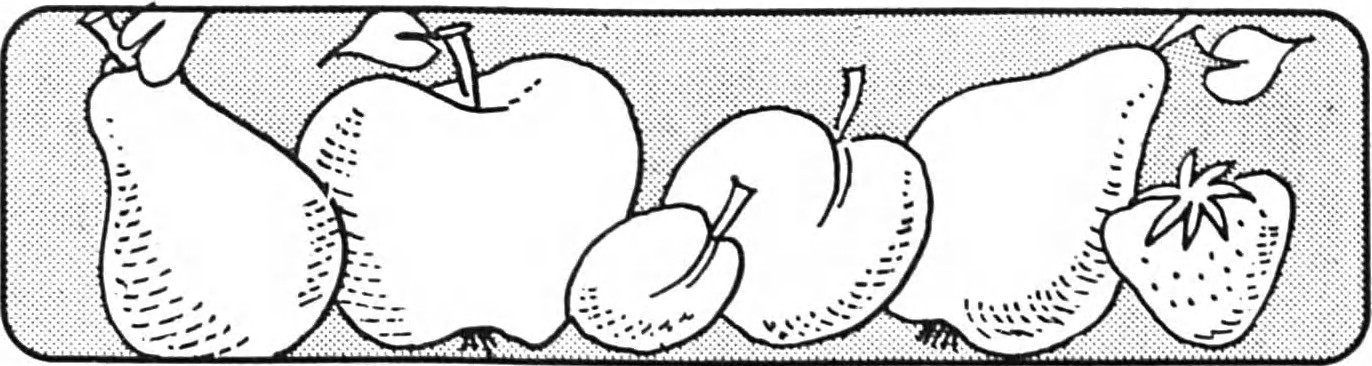
\includegraphics[width=\linewidth]{Images/EXP-1986-07-04-a-i0361.jpg}
    \end{subfigure}
    \hfill
    \begin{subfigure}{0.3\textwidth}
        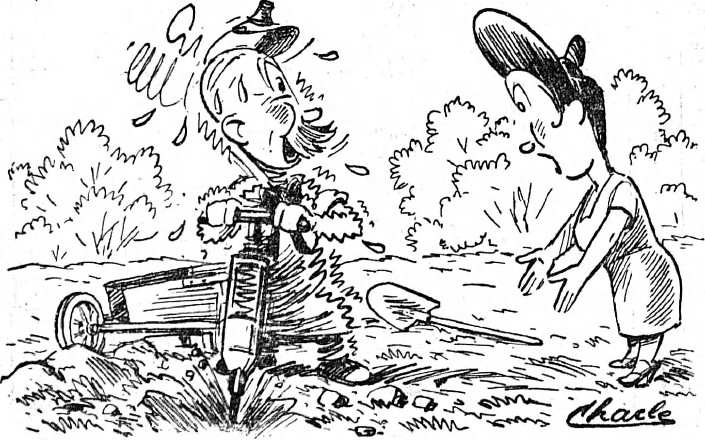
\includegraphics[width=\linewidth]{Images/IMP-1949-09-30-a-i0010.jpg}
    \end{subfigure}
    \hfill
    \begin{subfigure}{0.3\textwidth}
        
\includegraphics[width=\linewidth]{Images/IMP-1992-02-10-a-i0160.jpg}
    \end{subfigure}

    \caption{Drawings misclassified as comics before specifying that a drawing does not contain text.}
    \label{fig:3.7}
\end{figure} 

However, looking back at the misclassifications of comics as drawings, we see that they have increased from 10 to 22 instances. To attempt fixing this, we now specify in the prompt for the class \textbf{comic} that a comic does contain text. Thus, we modify the prompt from \textit{“entertaining traditional comic”} to \textit{“entertaining traditional comic \underline{including text}”}. Doing this decreases the misclassifications studied from 22 to 12 instances, as seen in Figure \ref{ig:CM-C}. A few images previously misclassified that are now classified correctly are shown in Figure \ref{fig:3.7}.

\begin{figure}[ht]
    \centering

    \begin{subfigure}{0.25\textwidth}
        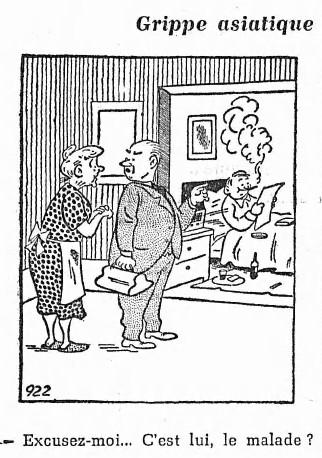
\includegraphics[width=\linewidth]{Images/IMP-1957-11-02-a-i0173_5.jpg}
    \end{subfigure}
    \hfill
    \begin{subfigure}{0.2\textwidth}
        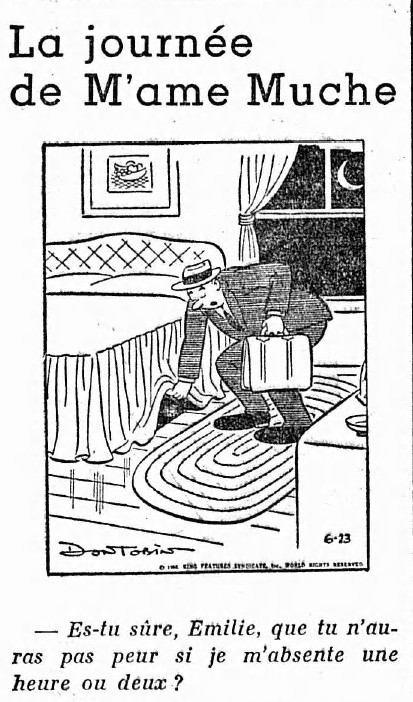
\includegraphics[width=\linewidth]{Images/EXP-1956-07-25-a-i0105.jpg}
    \end{subfigure}
    \hfill
    \begin{subfigure}{0.3\textwidth}
        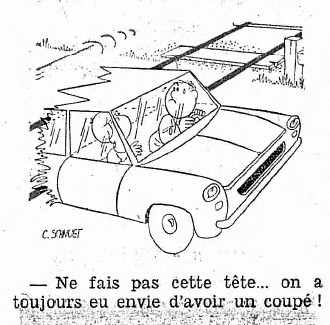
\includegraphics[width=\linewidth]{Images/IMP-1965-03-13-a-i0144_3.jpg}
    \end{subfigure}

    \caption{Comics misclassified as drawings before specifying that a comic contains text \\ \textit{and} a drawing does not contain text.}
    \label{fig:3.8}
\end{figure} 

%We also notice that even though the accuracy has increased, there are still misclassifications between the classes \textbf{comic} and \textbf{drawing}. These are due to: 
%Draft: Comment on the fact that the 8 misclassifications are drawings that contain text and show examples.\\

Implementing the lexical modifications stated above yields a new accuracy of \textbf{83.33\%}. From these results, we can conclude that \textbf{the prompts of the classes should be mutually exclusive}. 



\subsection{CLIP's multilingual abilities}

In this section, we explore CLIP's ability to generalise across languages, which is essential for its application in multilingual contexts and for inferring insights about the composition of its training data. To ensure a comprehensive evaluation, we selected a diverse range of languages from distinct families, as depicted in the leaves of the language tree shown in Figure \ref{fig:language-tree}. This approach allows us to investigate CLIP's performance across a variety of linguistic structures and vocabularies\footnote{The translations of the prompts were made using the Python \textit{translate} library \url{https://pypi.org/project/translate/}.}.

The languages chosen represent major families, each with its unique characteristics:

\begin{itemize}
    \item Sino-Tibetan: Represented by Mandarin, this family is known for its tonal nature and logographic writing system, providing a test for CLIP’s ability to handle non-alphabetic scripts and tonal distinctions.
    \item Slavic: With Russian as the representative, we aim to test CLIP's handling of Cyrillic script and the complex inflectional morphology typical of Slavic languages.
    \item Germanic: English and German from this family allow us to evaluate CLIP's performance in widely spoken languages with rich resources, possibly reflecting the model's training data.
    \item Latin: French and Spanish represent Romance languages derived from Latin, each with its own evolution and linguistic nuances.
    \item Semitic: Arabic and Hebrew, with their right-to-left script and root-based morphology, offer a distinct challenge, testing the model's capacity to deal with non-Latin scripts and unique linguistic structures.
\end{itemize}

% \clearpage
%improve formating and colours
\begin{figure}[ht]
\centering
\begin{forest}
  for tree={
    draw,
    align=center,
    font=\sffamily,
    edge={->},
    l sep=1cm,
    rounded corners=6pt, % Adjust the radius of rounded corners
  },
  [Language tree
    [Sino-Tibetan
      [Mandarin]
    ]
    [Slavic
        [Russian]
    ]
    [Germanic
        [German]
        [English]
    ]
    [Latin
      [French]
      [Spanish]
    ]
    [Semitic
      [Arabic]
      [Hebrew]
    ]
  ]
\end{forest}
\caption{Language tree.}
\label{fig:language-tree}
\end{figure}


%here should be a results section, same previously
\subsubsection{Results}

Our analysis reveals that English is the most proficient language, with German, Spanish, and French also demonstrating notably higher performance compared to the other assessed languages. German, belonging to the same Germanic family as English, achieves a peak performance of \textbf{64.69\%} using the \textit{specification} prompt, which is structured as \textit{“This” + class name + verb + preposition}.


\begin{figure}[ht]
    \centering

    \begin{subfigure}{0.31\textwidth}
        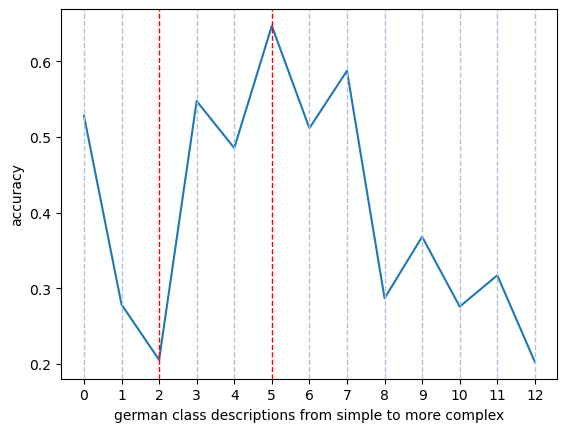
\includegraphics[width=\linewidth]{Images/germanacc.png}
    \end{subfigure}
    \hfill
    \begin{subfigure}{0.31\textwidth}
        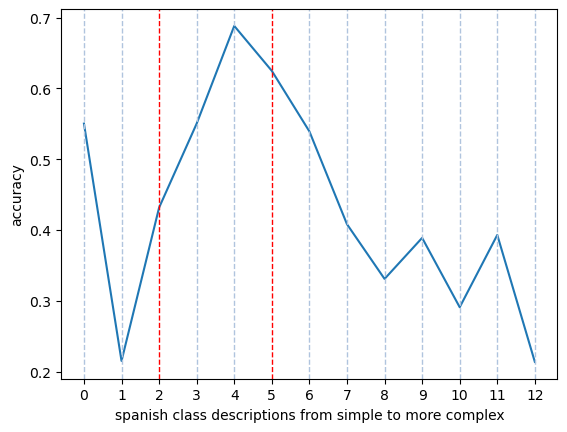
\includegraphics[width=\linewidth]{Images/spanishacc.png}
    \end{subfigure}
    \hfill
    \begin{subfigure}{0.31\textwidth}
        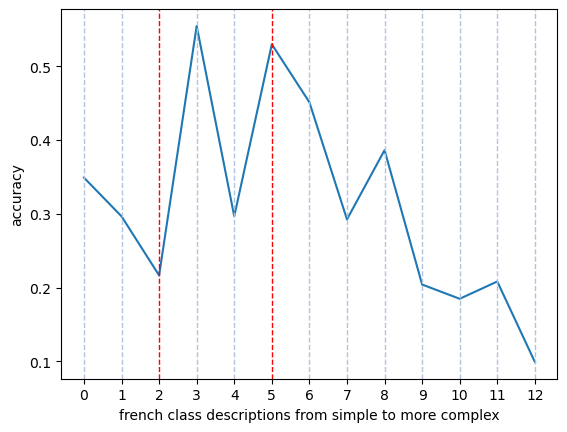
\includegraphics[width=\linewidth]{Images/frenchacc.png}
    \end{subfigure}

    \caption{Average accuracies across the thirteen prompts translated in German, Spanish and French.}
    \label{fig:lang-accs}
\end{figure} 


French and Spanish are both in the Latin family language. The peak performance is \textbf{68.83\%} for Spanish, using the \textit{disjunction of noun phrases} prompt, just like with the English prompts. As for French, it is \textbf{55.45\%}, using the \textit{noun phrases separated by comas} prompt.

It is noteworthy that the pattern observed in the previous section largely persists across these languages, with the specification prompt consistently emerging as the most effective across the three mentioned languages. This trend is further illustrated in Figure \ref{fig:lang-accs}, which showcases the average accuracy progression across the various prompts when translated into German, Spanish, and French.

Conversely, languages from the Sino-Tibetan, Slavic, and Semitic families did not perform as strongly, with their peak average accuracy hovering around \textbf{35\%}. Given this data, it is challenging to ascertain a clear pattern or identify the most effective prompts for these languages.

Based on these observations, it is reasonable to hypothesize that CLIP's training predominantly involved image and text pairs with text in Germanic and Latin languages. This insight could significantly influence future training and application strategies for multilingual vision-language models.

%arabic, hebrew not maintained 
%russian, mandarin roughly maintained 

%To identify the patterns visually, matrix with increases and drops in avg accuracy. one row per language. (class name as ref or english as ref? 
%<Insert Figure>
%- Are there interesting new repeated patterns?\\


\subsection{Discussion \& Conclusions}
In our analysis of CLIP's performance, we deduce that the model excels when presented with exhaustive and mutually exclusive prompts for classification tasks, suggesting a potential competitive edge against state-of-the-art fine-tuned models. A detailed comparison will be presented in a subsequent section of this report.

We also observed that the confidence level associated with CLIP’s predictions serves as a critical indicator of prompt effectiveness. Lower confidence levels are indicative of less accurate results, whereas higher confidence levels align with more accurate outcomes. This is a useful relationship for prompt engineering. Furthermore, our study highlights that CLIP exhibits optimal performance when prompted in English, which is likely reflective of the dominant language in its training data. While it demonstrates a reasonable understanding of Latin and Germanic languages, its proficiency diminishes significantly when confronted with other language families. 

% ----------------------------------------------------------------%

\section{Flamingo}

Flamingo is a model developed by Google DeepMind \parencite{alayrac2022flamingo}, which combines large language models with visual inputs designed to process both text and images simultaneously, allowing it to answer questions or perform tasks that rely on understanding both textual and visual information. The unique aspect of Flamingo is its ability to handle multimodal tasks that require understanding and integrating both text and visual data. This includes tasks like image captioning, visual question answering, and multimodal reasoning. Flamingo is built upon a foundation of large-scale Transformer-based language models. It extends these models' capabilities by including a mechanism for integrating visual information, essentially training the model to understand and process images in the context of related text.

\begin{figure}[ht]
  \centering
  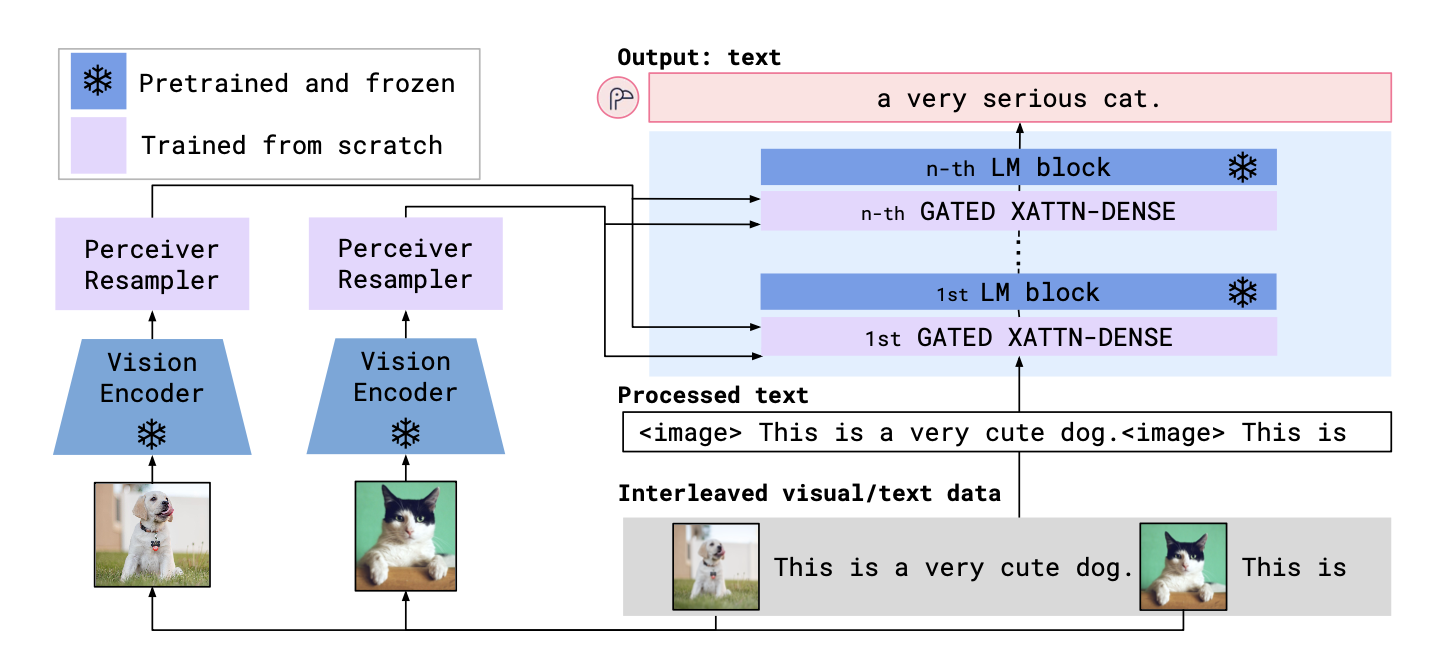
\includegraphics[width=0.8\linewidth]{Flamingo.png}
  \caption{Architecture of Flamingo from \cite{alayrac2022flamingo}.}
  \label{fig:flamingo}
\end{figure}
 
Its applications are broad and include performing tasks that require understanding the content of an image in the context of a question or description, explaining visual scenes, and answering questions that rely on both visual and textual understanding.


As presented in Figure \ref{fig:flamingo}, Flamingo works by accepting interleaved inputs in the form of text and images. The text is parsed from the inputs and the images replaced by placeholders. The images are then extracted from the input, parsed through a frozen vision encoder, then mapped through the perceiver resampler to produce a fixed number of visual tokens per input. The tokens are used as inputs to cross attention layers to condition a language model that has taken as input the text sequence. The model finally proceeds with the completion of the partial text. It is worth noting that the vision encoder is pretrained as a dual encoder using contrastive loss employed by CLIP.

Flamingo is a particularly interesting model to study because of its flexible architecture. In fact, CLIP's architecture lacks flexibility, in the sense that the model can select the best image and text pairings, but does not have the ability to generate language. It is thus not suited for open-ended tasks like captioning or visual question answering. Flamingo, on the other hand, is able to perform open-ended tasks. We will particularly explore its captioning capabilities later in this report. But first, we explore its classification abilities.

\paragraph{Hyperparameters} For the implementation of Flamingo, since the model is not open-sourced by DeepMind Google, we worked with the unofficial implementation by \cite{mlfoundations2022openflamingo}, \parencite{openai2022clip-repo} and took inspiration from the \parencite{lucidrains2022flampytorch} repository.

%Draft:Moreover, we can try few-shot

\subsection{Prompting Flamingo for zero-shot \& few-shot image classification}

It is possible to perform classification using Flamingo by inserting the class name into text templates of the form “a photo of a \textit{class}”, then selecting the text that is assigned the highest similarity to the image embedding by the model. This is done using maximum likelihood. However, since this would be equivalent to repeating the same experiment as previously done with CLIP, we focus on evaluating the generative capabilities of Flamingo.

To facilitate this, we employ four distinct types of prompts, each designed to elicit a specific kind of response from Flamingo. These prompts are the beginnings of sentences that the model will complete, providing predictions that can be post-processed to extract class information. 

\begin{table}[ht]
    \centering
    \begin{tabular}{cl}
        \rowcolor{lightgreen} \textbf{Index} & \textbf{Prompt} \\
        \rowcolor{lightgreen} 1 & “An image of” \\
        \rowcolor{lightgreen} 2 & “This image can be classified as” \\
        \rowcolor{lightgreen} 3 & “Keywords describing this image are” \\
        \rowcolor{lightgreen} 4 & “The type of this image is” \\
    \end{tabular}
    \caption{Prompt variations for classification using Flamingo.}
    \label{tab:flam-prompts}
\end{table}

The prompts are outlined in Table \ref{tab:flam-prompts} and explained below:
\begin{itemize}
    \item \textit{“An image of”}: This is a simple and open-ended prompt, recommended by \parencite{alayrac2022flamingo}, encouraging the model to freely describe what it sees in the image. The generative nature of Flamingo can lead to diverse responses, which can then be analysed to infer the image's class.
    \item \textit{“This image can be classified as”}: This prompt is more direct and asks the model to categorize the image explicitly. It is designed to assess how well Flamingo can perform explicit classification tasks in a generative manner.
    \item \textit{“Keywords describing this image are”}: By asking for keywords, this prompt aims to extract specific descriptors from Flamingo that can be indicative of the image's class. This can be particularly useful for understanding the model's perception and the primary elements it focuses on when viewing an image.
    \item \textit{“The type of this image is”}: Similar to the second prompt, this one also seeks a direct classification. However, the slight variation in wording allows us to compare the effects of phrasing on Flamingo's classification accuracy and consistency.
\end{itemize}


%Draft: Mention the patterns observed, the consistent mistakes and weird behaviours etc.

\paragraph{Flamingo Answer Post-processing} The post-processing strategy employed consists in transforming the original captions into a single-word representation corresponding to the predicted class. Given a single caption, the algorithm iterates through each word and maps it to the appropriate class based on a predefined dictionary shown in Table \ref{tab:dic}. 

\begin{table}[ht]
    \centering
    \begin{tabular}{|l|l|}
        \hline
        \textbf{Class} & \textbf{Keyword list} \\
        \hline
        drawing & drawing, illustration, fashion, ornamental, cartoon \\
        \hline
        game & puzzle, sudoku, chess, crosswords, poker, card games, grid, wordsearch \\
        \hline
        graph & chart, graph, plot, histogram, diagram, graphic \\
        \hline
        logo & logo, ad, advertisement, publicity, symbol, label, emblem \\
        \hline
        comic & comic, cartoon \\
        \hline
        map & map, blueprint, plan \\
        \hline
        photo & photograph, photo, view, close-up \\
        \hline
        title & title, letter, C, O, N, F, E, D, R, Confédéré, monogram\\
        \hline
    \end{tabular}
    \caption{Dictionnary used for the post-processing of predictions.}
    \label{tab:dic}
\end{table}

This dictionary was created based on the class descriptions made when the dataset was annotated by \cite{dhlab2022impresso}, and by interactively adding synonyms when observing the model’s responses. Subsequently, it handles all possible cases of duplicated or conflicting classes. There could be more than one predicted class if the caption contains keywords from different classes. In this case, if one of them is \textit{drawing}, then the algorithm chooses the other class. This is because, as stated earlier, many classes are subsets of a \textit{drawing}. For example, a comic is a drawing, but a drawing is not necessarily a comic.

Otherwise, the algorithm chooses the class that has the maximum number of occurrences, if there is such a class. If not, the algorithm dynamically prompts Flamingo to settle between the classes, ensuring a more accurate and refined result. The prompt used to do so is the following: 
 “\textit{Between the classes \blank{} and \blank{}, this is a}”.
 
It recursively processes the new generated prompts, following this same algorithm. This strategy is applied to all generated captions, and aims to enhance the precision of the model's classification output by intelligently handling ambiguities and optimizing the query prompts for improved results.
% \clearpage



\subsubsection{Results}
Prompting Flamingo with a 0-shot prompt highlights its proficiency in describing an image concisely, and with precise words. This is being reflected in a very high precision for all classes. However, we observe a very low recall since the generated texts are so distinctive that it is hard to include all possible keywords in a dictionary. For this reason, there are a lot of misclassifications. This particularly happens for the class \textit{photo} since the model describes what it sees on the photograph instead of recognizing that it is a photograph. Prompt 2, namely \textit{“This image can be classified as”} mitigates this behaviour since it explicitly asks to \textit{classify} the image, to which the model sometimes responds \textit{photograph}. Concerning the 0-shot experiment on prompt 2, there is a total of 202 out of 725 unclassified images, 114 of which are photographs, and only 53 misclassifications. The repartition of these misclassifications can be seen in Figure \ref{fig:cm-p2-0s}. 

This behaviour immediately changes when inputting few-shot prompts. As illustrated in Figures \ref{fig:cm-p2-1s} and\ref{fig:cm-p2-2s}, the misclassifications increase significantly, as the number of unclassified images decreases from 202 to 185 in 1-shot, then to 0 in 2-shots. On the other hand, misclassifications increase from 53 to 332 to 680 in 2-shots, where all images are classified as logos. Looking at all few-shot results across prompts, it seems that Flamingo picks up on the pattern of the prompt but fails to complete it correctly.
%TODO: run 2 shot for prompt 3 and 4 and see if it's better or worse than 1-shot

\begin{figure}[ht]
    \centering

    \begin{subfigure}{0.31\textwidth}
       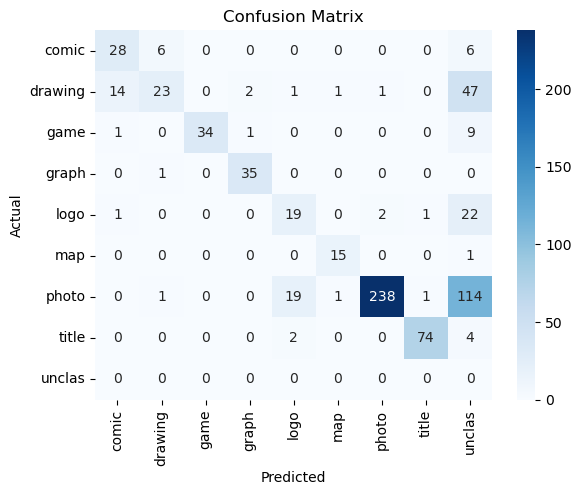
\includegraphics[width=\linewidth]{Images/cm-flam-p2-0s.png}
        \caption{0-shot}
        \label{fig:cm-p2-0s}
    \end{subfigure}
    \hfill
    \begin{subfigure}{0.31\textwidth}
        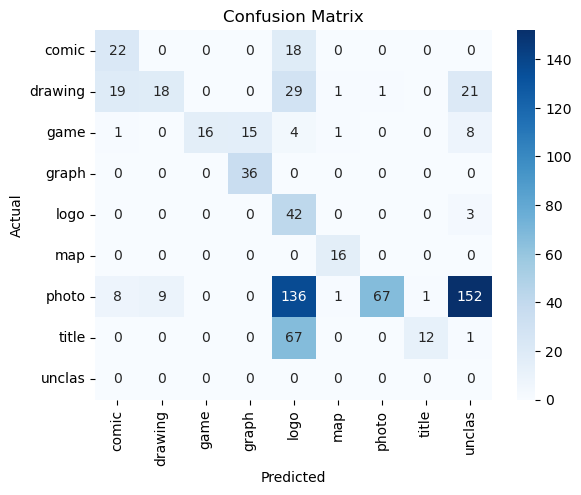
\includegraphics[width=\linewidth]{Images/cm-flam-p2-1s.png}
        \caption{1-shot}
        \label{fig:cm-p2-1s}
    \end{subfigure}
    \hfill
    \begin{subfigure}{0.31\textwidth}
        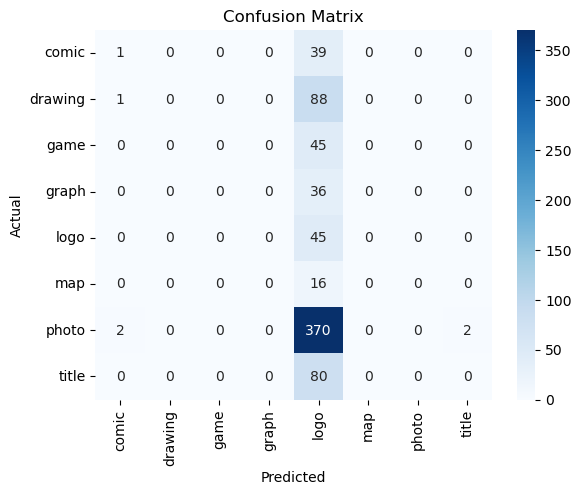
\includegraphics[width=\linewidth]{Images/cm-flam-p2-2s.png}
        \caption{2-shot}
        \label{fig:cm-p2-2s}
    \end{subfigure}

    \caption{Confusion matrices across number of shots prompting Flamingo with \textit{"This image can be classified as a"}.}
    \label{fig:avg-acc-trans}
\end{figure} 

We choose to look at the macro-average to assess the results, presented in Table \ref{tab:overall-flam-res}, since it provides a balanced view of performance across all classes.

\begin{table}[ht]
    \centering
    \begin{tabularx}{\textwidth}{|X|r|r|X|X|}
        \hline
        \textbf{Prompt} & \multicolumn{2}{c|}{\textbf{Macro-average}} \\
        & \textbf{0-shot} & \textbf{1-shot} & \textbf{2-shot} \\
        \hline
        1 & 48.97\% & 41.49\% & 25.84\%  \\
        \hline
        2 & 65.82\% & 43.04\% & 2.04\% &  \\
        \hline
        3 & 43.45\% & 55.79\% &  38.52\% &  \\
        \hline
        4 & 42.94\% & 56.03\% &  20.26\% &  \\
        \hline
    \end{tabularx}
    \caption{Macro-average per prompt using Flamingo.}
    \label{tab:overall-flam-res}
\end{table}

%draft: What made such a big difference for prompt 4 is that it recognized photo which has the highest support. this doesn't hold anymore because macro-avg and not acc ?




\subsection{Discussion \& Conclusions}
To gain more insights on the capabilities of Flamingo and its behaviour, we perform a quantitative and a qualitative analysis of the texts it generated. The predicted texts are displayed on the table accessible at \url{https://github.com/dh-epfl-students/dhlab-image-captioning/blob/main/FLAMINGO/class_summary.html)}.

\subsubsection{Quantitative Analysis}

The quantitative analysis performed here focuses on the frequency of the texts predicted by Flamingo. Since all images are different, it is likely that the captions are distinct even if two images belong to the same class. The desired behaviour is that the number of different captions decreases as we increase the number of shots. We observe in Figure \ref{fig:freq-plot} that this is indeed what happens, however, the performance decreases as seen in the previous section.

\begin{figure}[ht]
    \centering

    \begin{subfigure}{0.31\textwidth}
        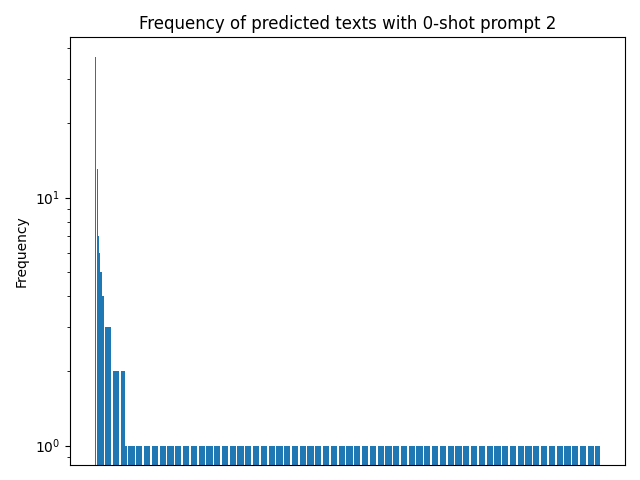
\includegraphics[width=\linewidth]{Images/0-shot_prompt_2_freq_plot.png}
    \end{subfigure}
    \hfill
    \begin{subfigure}{0.31\textwidth}
        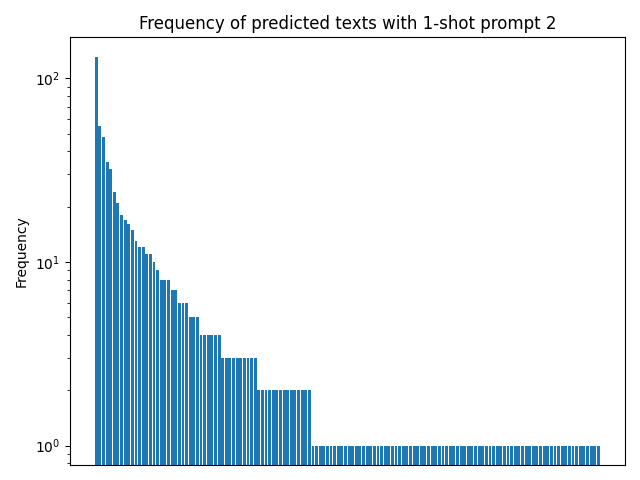
\includegraphics[width=\linewidth]{Images/1-shot_prompt_2_freq_plot.png}
    \end{subfigure}
    \hfill
    \begin{subfigure}{0.31\textwidth}
        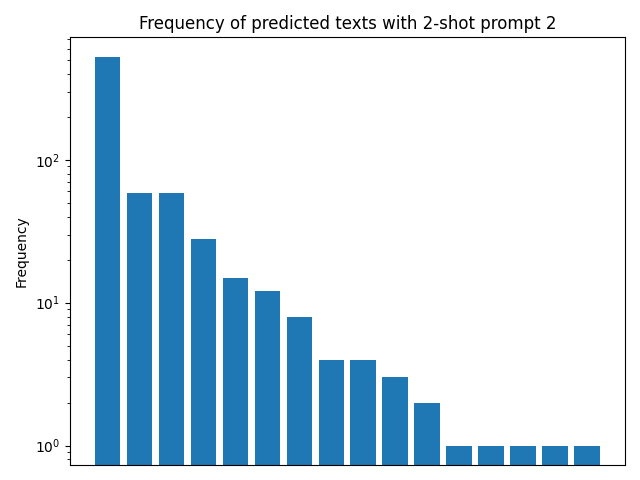
\includegraphics[width=\linewidth]{Images/2-shot_prompt_2_freq_plot.png}
    \end{subfigure}

    \caption{Frequency of prompts on 0-shot, 1-shot and 2-shot using the prompt \textit{"This image can be classified as a"}.}
    \label{fig:freq-plot}
\end{figure} 

We also notice that, as we increase the number of shots, the generated texts become more repetitive. The top-3 repeated texts across number of shots on prompt 2 are shown in Table \ref{tab:top-preds}.


%separate row with lines
\begin{table}[ht]
    \centering
    \begin{tabular}{|p{2.5cm}|p{6cm}|p{6cm}|}
        \hline
        \rowcolor{lightgray}\textbf{0-shot} & \textbf{1-shot} & \textbf{2-shot}\\
        \rowcolor{white} crossword puzzle & This image can be classified as a logo. & This image can be classified as a logo. This image can be classified as a game. This image can be classified\\
        \rowcolor{white} comic strip & This image can be classified as a logo. This image can be classified as a painting. This image can be classified & This image can be classified as a comic. This image can be classified as a logo. This image can be classified\\
        \rowcolor{white} bar graph & This image can be classified as a photograph & This image can be classified as a graph. This image can be classified as a logo. This image can be classified\\
        \hline
    \end{tabular}
    \caption{Top 3 predictions across the number of shots for the prompt \textit{"This image can be classified as a"}.}
    \label{tab:top-preds}
\end{table}


\subsubsection{Qualitative Analysis}

When looking at the generated texts, we notice that for the same image, the model generates a sequence of different predictions following the prompt pattern, for example: “This image can be classified as a logo. This image can be classified as a game. This image can be classified". This is an undesired behaviour and can hypothetically be explained by the fact that few-shot prompting confuses the model by making the prompt very long.

We can confidently assert that the model detects well the elements of an image, and can differentiate between objects, people and animals. However, it lacks the ability to generate mutually exclusive predictions, for example: “This image can be classified as a graph. This image can be classified as a logo”. Moreover, it could benefit from a better understanding of the prompt and the context. It should recognize that the sentence completion is expected to provide a single, coherent suggestion rather than a list of possibilities.

\section{Comparing CLIP, Flamingo, and VGG-16} 

VGG-16 is a convolutional neural network architecture that was a notable development in the field of deep learning and computer vision, and it achieved high levels of accuracy in the ImageNet competition, which is a benchmark in image classification and recognition.

We compare the three models' best performance against each other. For VGG-16, the result presented in Table \ref{tab:comparison} was obtained by training the model on the dataset using an SGD optimizer, with batch size 32 and learning rate 0.01 \parencite{dhlab2022impresso}. On the other hand, CLIP's result was obtained by prompting the model with disjunction of noun phrases on a closed-ended task. Finally, the result using Flamingo was achieved by prompting Flamingo on an open-ended task, inputting \textit{"This image can be classified as a"} and post-processing the predictions to map them to the desired classes. It is important to mention that the results obtained using VGG-16 were achieved on the complete dataset, i.e. including the classes \textit{diverse} and \textit{other}, which were omitted in the context of our experiments on CLIP and Flamingo.

\begin{table}[h]
    \centering
    \begin{tabularx}{\textwidth}{|l|r|r|r|}
        \hline
        & \textbf{VGG-16} & \textbf{CLIP} & \textbf{Flamingo} \\
        \hline
        \textbf{Average accuracy} & \bf 89.14\% & 83.33\% & 64.28\% \\
        \hline
    \end{tabularx}
    \caption{Comparison table of average accuracies.}
    \label{tab:comparison}
\end{table}

\section{Conclusions}

Upon examining the generated texts, a notable observation is the model's tendency to produce diverse predictions for the same image when prompted in a few-shot manner. This behaviour, seemingly triggered by the length of the prompt, is undesirable and requires further investigation.

Moving forward, our comparison of CLIP, Flamingo, and VGG-16 sheds light on their respective strengths and weaknesses. For CLIP to compete with fine-tuned models, it should be prompted optimally, following the patterns we have recognised to be effective through our experiments. This requires some prompt engineering, and opens up the possibility of an automatised way of improving the prompts. On the other hand, since classification results were derived from prompting Flamingo on an open-ended task, they underscore the true classification capability of the model, but offer us more understanding of its strengths and limitations.